\documentclass[12pt]{article}

\counterwithin{figure}{section}
\counterwithin{table}{section}
\counterwithin{equation}{section}

\usepackage{blindtext}
\usepackage{graphicx}
\usepackage{listings}
\usepackage{float}
\usepackage{cite}
\usepackage{amsmath}
\usepackage{amssymb}
\usepackage{booktabs}
\usepackage{fullpage}
\usepackage{color}
\usepackage{url}

\definecolor{dkgreen}{rgb}{0,0.6,0}
\definecolor{gray}{rgb}{0.5,0.5,0.5}
\definecolor{mauve}{rgb}{0.58,0,0.82}

\lstset{frame=tb,
  language=Python,
  aboveskip=3mm,
  belowskip=3mm,
  showstringspaces=false,
  columns=flexible,
  basicstyle={\small\ttfamily},
  numbers=none,
  numberstyle=\tiny\color{gray},
  keywordstyle=\color{blue},
  commentstyle=\color{dkgreen},
  stringstyle=\color{mauve},
  breaklines=true,
  breakatwhitespace=true,
  tabsize=4
}

\title{KD trees in ray tracing}
\author{Miloš Medić}
\date{January 2023.}

\begin{document}
\maketitle
\thispagestyle{empty}

\newpage
\tableofcontents
\thispagestyle{empty}

\clearpage
\pagenumbering{arabic}
\section{Introduction}
Computer graphics is one of the fastest growing fields of computer science today. This is because it has direct practical implications to the way we view media on a screen. One big subfield of it is ray tracing. Ray tracing is the act of casting rays onto a 3D scene to calculate how it should look on a 2D screen \cite{glassner1989introduction}. Major advances are constantly being made in the field, like the recent ReSTIR algorithm \cite{ouyang2021restir}. \\
\indent One major topic in the field are acceleration structues. Acceleration structures are data structures used to group polygons (usually triangles) so that we can check if a specific ray intersects with some polygon in the scene, and if so, which one \cite{glassner1989introduction}. A single scene could contain hundreds of thousands to millions of triangles and a similar number of rays could be cast, so these data structures make a huge difference. Some popular ones are uniform grids, quadtrees (and octrees), binary space partitioning trees, KD trees, and bounding volume hierarchies. These data structures have other uses, related to computer graphics, like quadtrees in terrain destruction \cite{nassen2019real}, and not related, like KD trees in range searching. In this paper we will cover KD trees and how they can be used in ray tracing.

\section{Space partitioning motivation}
%\includegraphics[settings]{file}
How does grouping triangles with acceleration structures lead to higher performance? Let us explain this through an example. Suppose we want to render a scene with 1080p resoution. That is $1920 \times 1080 = 2,073,600 \approx 2 \cdot 10^6$ pixels. If we cast a ray through each one, that is approximately $2 \cdot 10^6$ rays. Suppose we have $100,000=10^5$ triangles in our scene. Now for each of the rays we need to know what the first triangle it intersects with is. To calculate the pixel color values for a corresponding ray, we need to know the angle at which it intersects the triangle, the color of the triangle, the texture of the triangle, etc.\footnote{In reality a pixels color value may not be calculated from just one ray, the fact that we still need the information about the first intersecting triangle still stands.} It is trivial to check whether a single ray intersects a particular triangle, but to know which triangle it intersects first, if any at all, is a much more difficult problem. The naive approach would be to check all rays against all triangles in the scene. This would result in $2\cdot10^6\times10^5=2\cdot10^{11}$ checks. That is assuming no ray continues bouncing after the first intersection, which it might do in some ray tracing algorithms. Suppose that we split the scene spatially in half with a plane, such that the number of triangles to the left of the plane $N_l$ is similar to the number of triangels to the right $N_r$, $N_l \approx N_r$, see Figure \ref{figure:sp}.\\
\begin{figure}[!h]
\centering
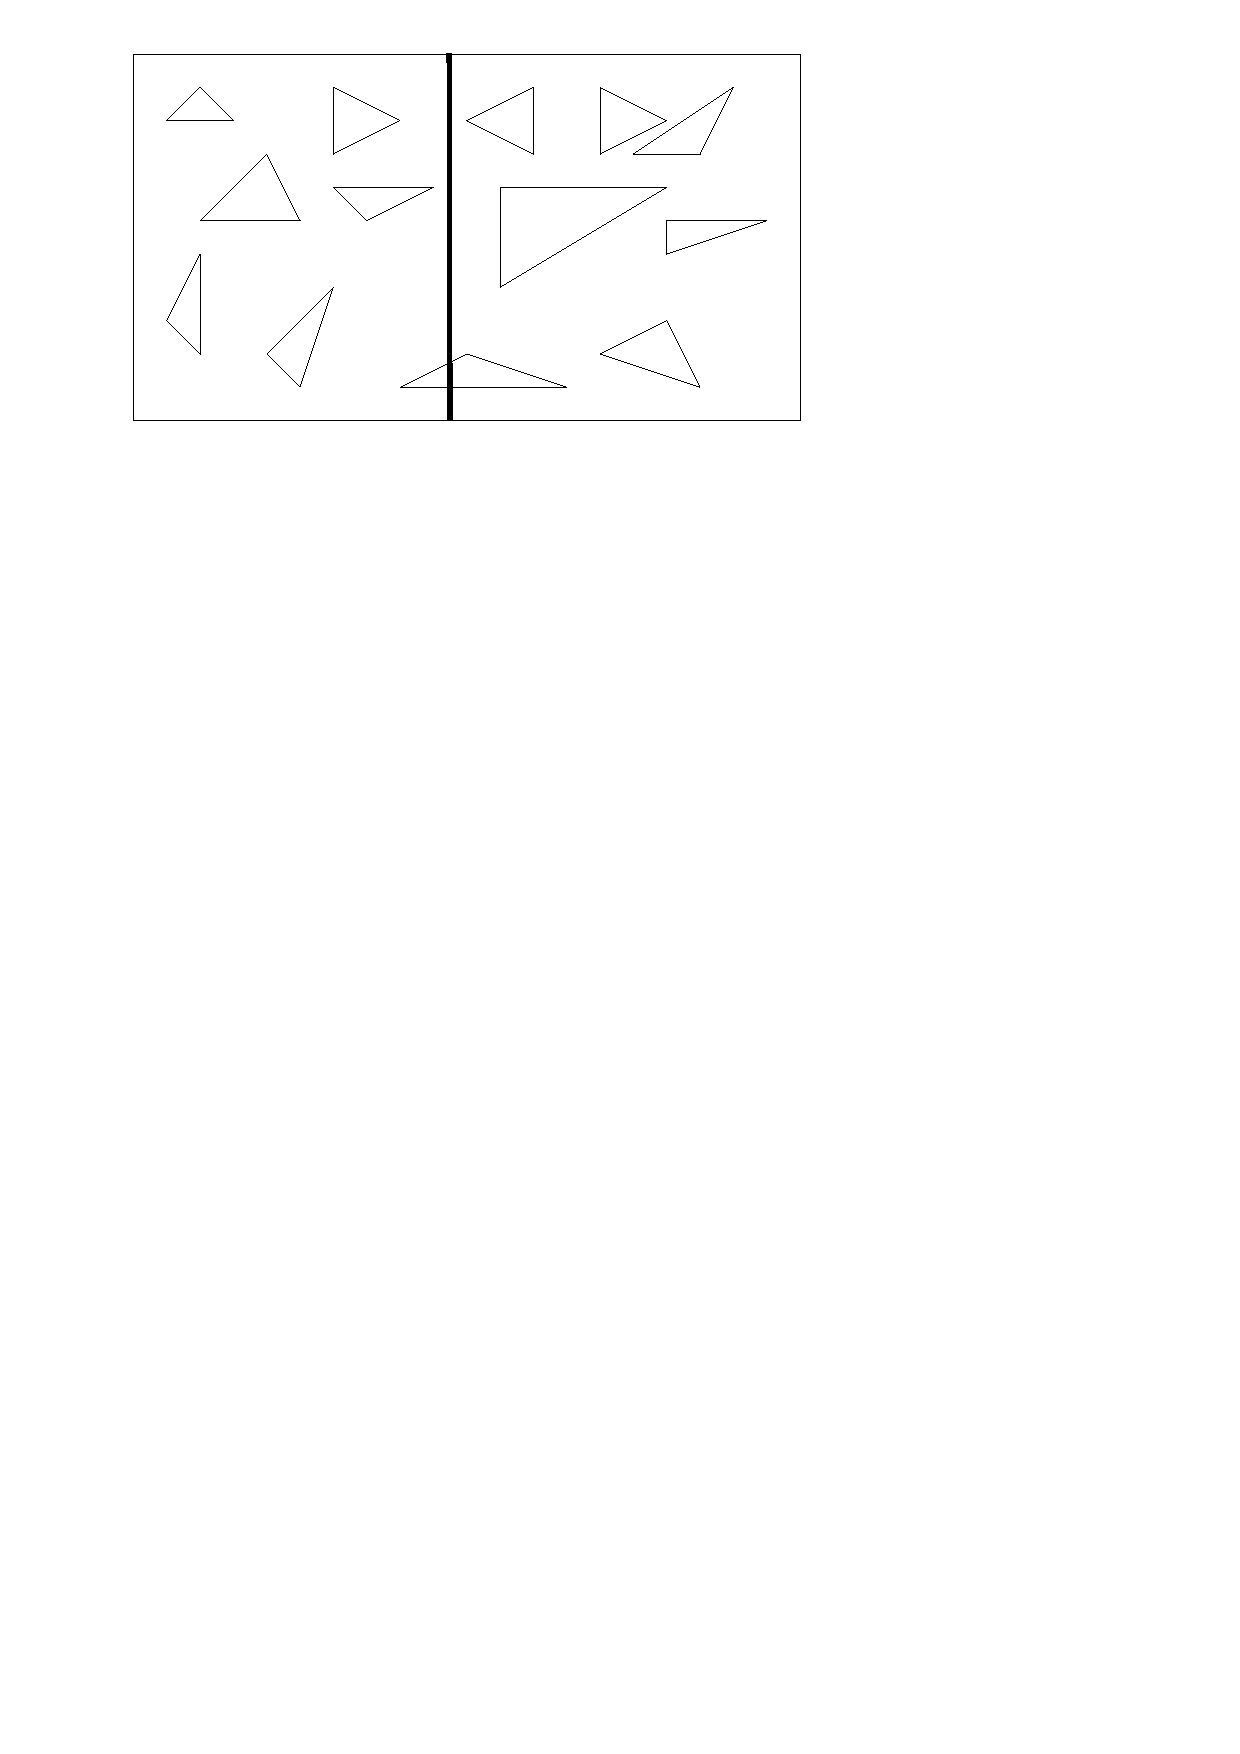
\includegraphics{figs/splittingPlane}
\caption{\textit{A 2D scene being split in half by a line. The figure is scaled one dimension down (2D scene split by a line) for visual clarity.}}
\label{figure:sp}
\end{figure}
\indent We can count any triangles that intersect the plane, in both $N_l$ and $N_r$. Let us say that $N_l=N_r=\frac{10^5}{2}=5\cdot10^4$. Now for each ray, we first check if it intersects with the space to the left of the plane (containing $N_l$ triangles) or to the space to the right of the plane (containing $N_r$ triangles). Then for a ray that does not intersect both spaces we just have to check it against $N_l$ or $N_r$ triangles, not $N_l + N_r$ like before. In this instance, since we assumed $N_l=N_r$ every ray would have to commit $1 + 5\cdot10^4$ intersection tests for a total of $2\cdot10^6\times(1 + 5\cdot10^4)=100,002,000,000\approx10^{11}$ checks. This is half the checks we had to do before, which will greatly improve the rendering time for the frame. 
We may continue splitting the 3D space like this into subgroups. For each ray we first find which subspace it belongs to (it is important that the subspaces are mutually excslusive), and then we just check against all triangles in the subspace. The more we divide the space the more checks we have to do to find out what subspace a ray belongs to, but we will have less triangles in the subspace to do checks against. Acceleration structures tell us how to divide the space, and usually give us a method of finding in which subspace a ray is in that does not constitute checking against every single subspace. Often, they let us go down a hierarchy. \\
\indent Note that we can also generalize this concept of splitting the space to higher (and lower) dimension spaces than 3D, where we split a space of dimension $d$ with a space of dimension $d - 1$. This $d - 1$ dimensional object is then called a hyperplane \cite{rockafellar1970convex}. A hyperplane for three dimensions is called a plane, for two dimensions it is a line, for one it is a point.

\section{Binary Space Partitioning}
\subsection{The general definition}
KD trees are a type of Binary Space Partitioning trees (BSP trees). BSP trees are called binary since they continually divide the space into two. In contrast Quadtrees continually divide 2D space into 4, Octrees continually divide 3D space into 8, and Bounding Volume Hierarchies (BVHs) continually take some number of subspaces from the current space, which do not even have to be a partition of the original space. These data structures are detailed in \cite{ericson2004real}. \\
More precisely we construct a BSP tree in the following way:

\begin{lstlisting}
function buildBSPTree(currentNode):
	if MeetsStoppingCriteria(currentNode)
		return
	plane = GetSplittingPlane(currentNode)
	(leftChild, rightChild) = SplitSpace(currentNode, plane)
	currentNode.leftChild = leftChild
	currentNode.rightChild = rightChild
	buildBSPTree(leftChild)
	buildBSPTree(rightChild)
\end{lstlisting}

The function buildBSPTree would be called on the root node which usually represents the Axis Aligned Bounding Box (AABB) of all the triangles. \\
\indent The union of the two subspaces of a node is equivalent to the space the node represents. The union of all the leaves of the tree is the space represented by the root, the AABB. The subspaces represented in the children of a node are mutually exclusive, but the sets of polygons (in our context triangles) they contain may not be. This is because some polygons can intersect the plane, or even be fully contained by it. We can make the sets of polygons mutually exclusive by dividing them, and putting their parts in their respective sets. We can put the polygons fully contained in the plane into any of the two sets.\\
\indent We want to find out which ray intersects which leaf of the tree. We do this by traversing the tree, we check if a ray intersects with the space represented by the left or by the right child of a node, starting with the root, and continue the process recursively until we hit a leaf. If the ray intersects both subspaces we can just choose one to traverse, in the context of ray tracing this is the subspace the ray hit first.

\subsection{KD trees}
KD trees, i.e. $k$-dimensional trees, constrict BSP trees so that every hyperplane has to be axis-aligned. This constriction is useful since even finding an appropriate axis-aligned hyperplane is computationally expensive. Adding another degree of freedom (that BSP trees have) can really limit the usefulness of the data structure due to its time-costly construction, and not at a great benefit at that. That being said there have been some successful attempts at using non-axis-aligned BSP trees in ray tracing \cite{ize2008ray}. It is also common that the axis with which the hyperplane is aligned is changed cyclically as stated in the paper that invented the algorithm \cite{bentley1975multidimensional}. So for 3D the aligning axis would be: $x$, $y$, $z$, $x$, $y$, $z$, $x$.... as we go down the tree, though it can start with any axis, not just x. The splitting axis is sometimes referred to as the \textit{discriminator} in the literature.

\subsubsection{Use cases}
In the original paper by Jon Louis Bentley\cite{bentley1975multidimensional} the data structure was invented to help manage data with arbitrary dimensionality. In particular it was to allow queries on data which had records of the form of a $k$-tuple $(v_0, v_1, \dots, v_{k-1})$. The algorihms for node insertion, deletion, tree construction, and tree traversal for search queries are described. One of the most obvious uses is for range searching \cite{bentley1975multidimensional}. For a range search we can specify in what range we want to look for entries in the tree. Here it can be useful to visualize the data.
\begin{figure}
\centering
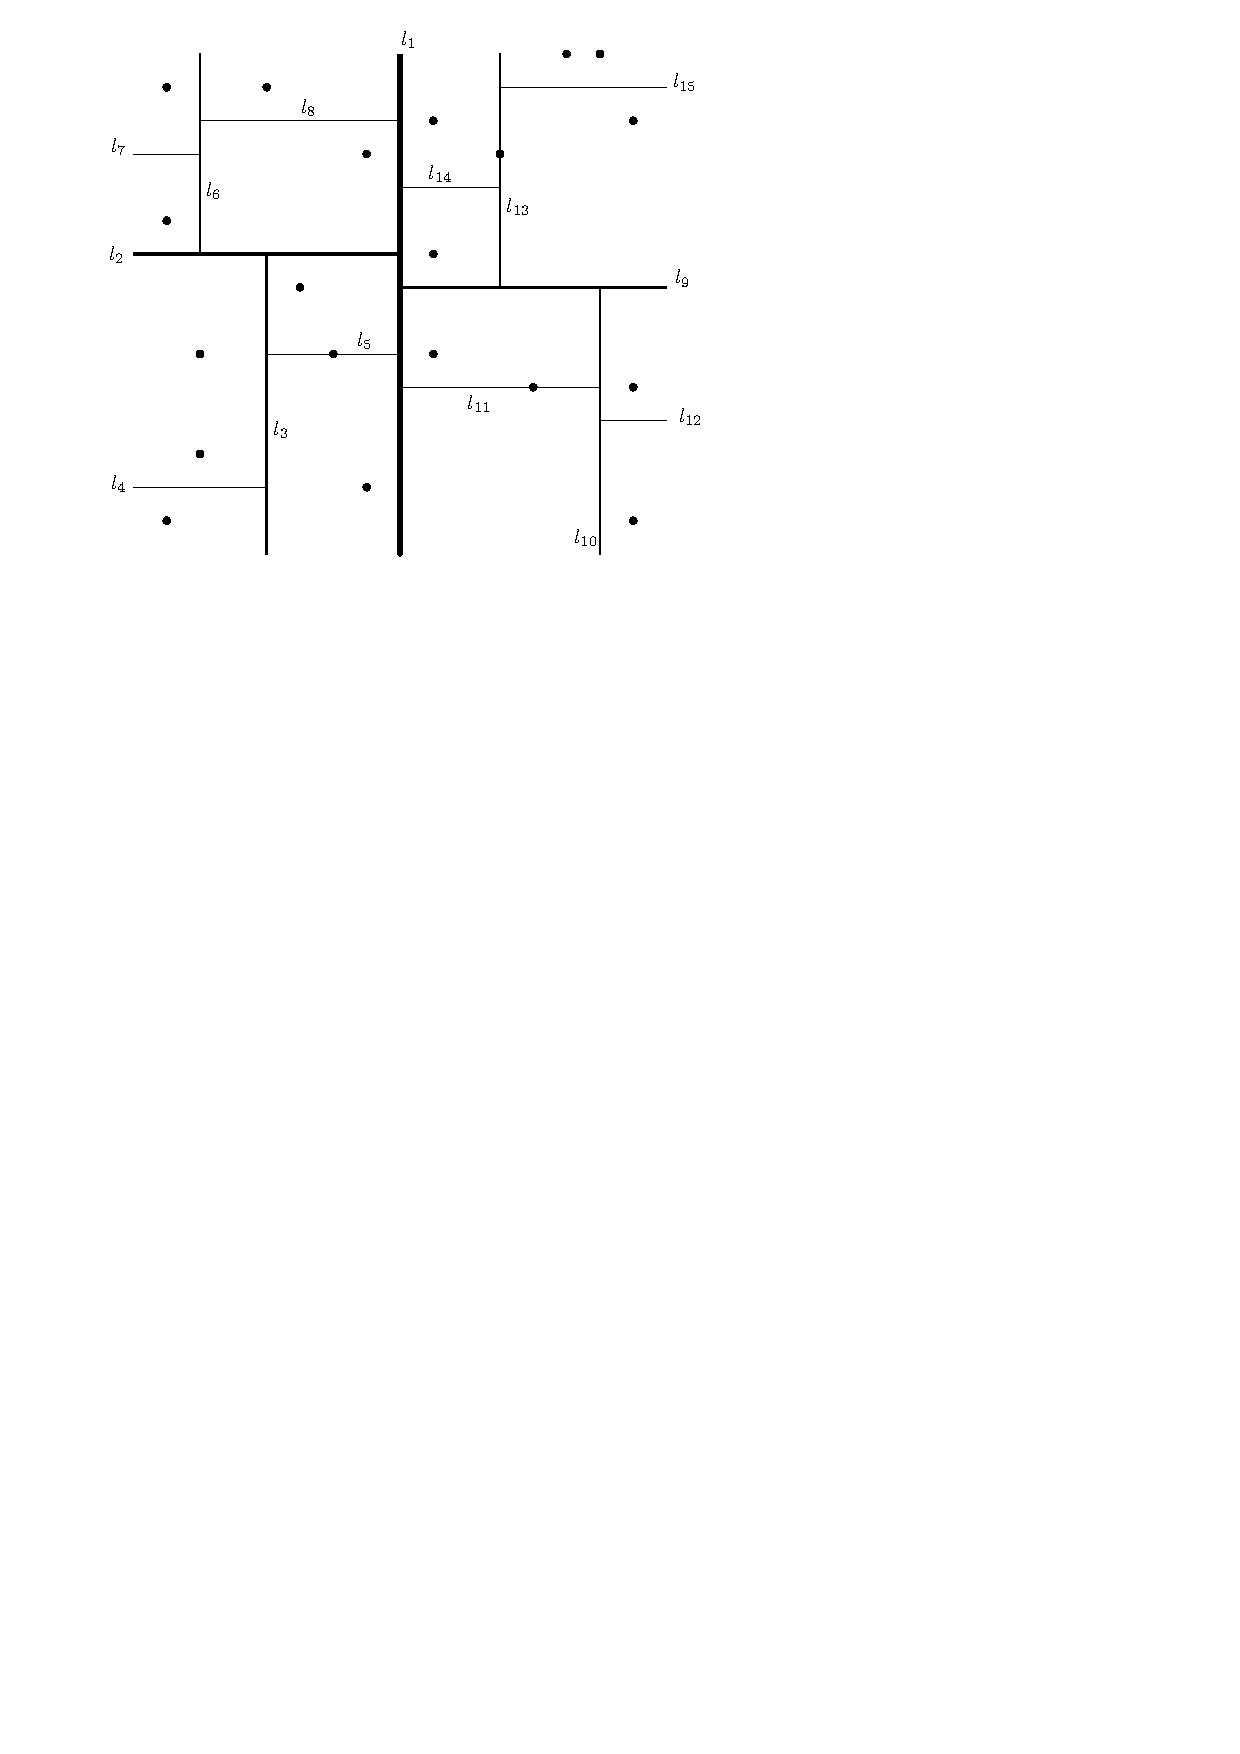
\includegraphics{figs/kdTreePlane}
\caption{\textit{A 2D space subdivided by a KD tree.}}
\label{figure:kdp}
\end{figure}
\begin{figure}
\centering
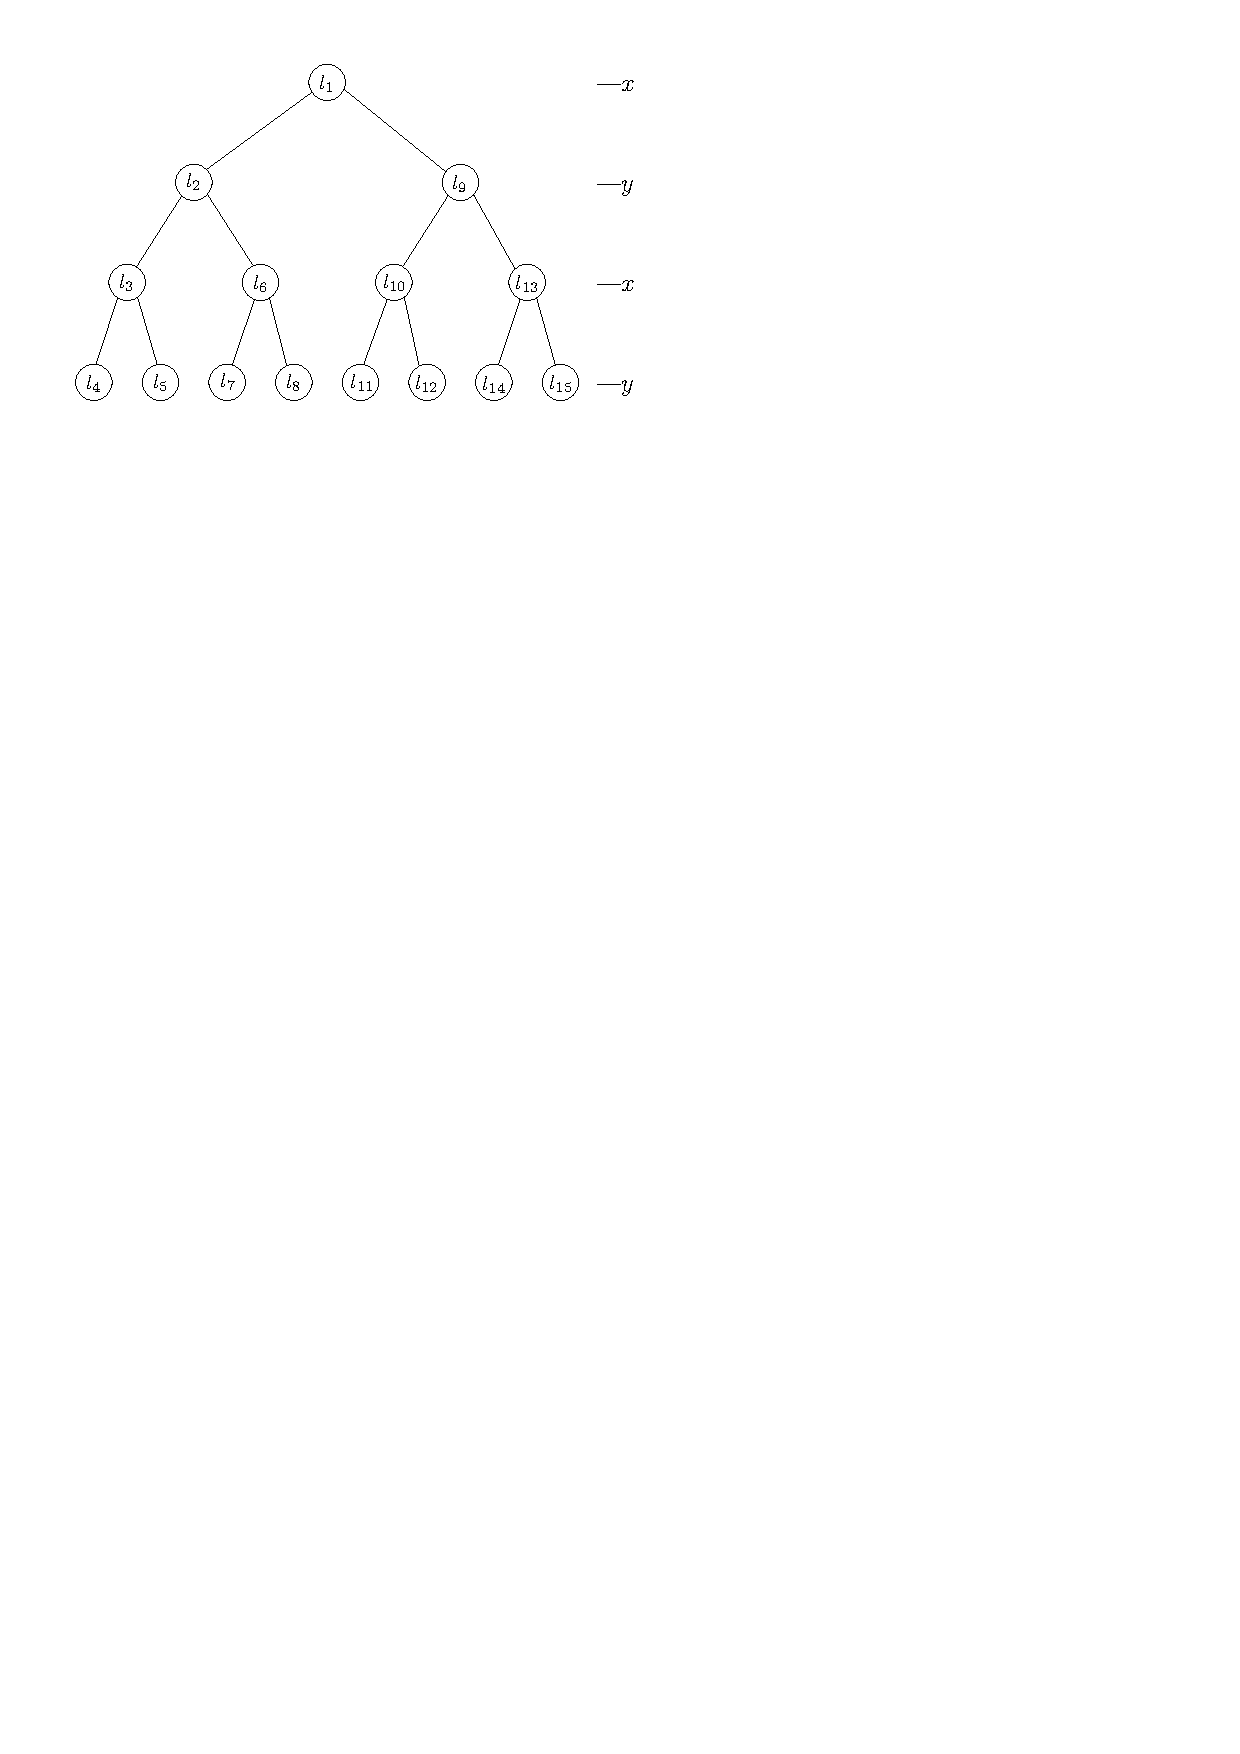
\includegraphics{figs/kdTree_updated}
\caption{\textit{The KD tree in Figure \ref{figure:kdp}. with its vertices marked with the split lines.}}
\label{figure:kdt}
\end{figure}
In Figure \ref{figure:kdp}, the space is divided by 15 lines, representing the splits in the tree nodes. The thinner the lines the deeper they are in the tree. We can also see that the lines alternate between splitting the x and the y dimension. The data points are depicted as points in the figure. Each has a corresponding x and y coordinate. If we look at Figure \ref{figure:kdt} we can see that the lines were labeled so that the index corresponds to the order in which they will most likely be created following the recursion. If we imagine an AABB encompasing Figure \ref{figure:kdp}, each of the small regions is represented by a leaf in the tree in Figure \ref{figure:kdt}.
\begin{figure}
\centering
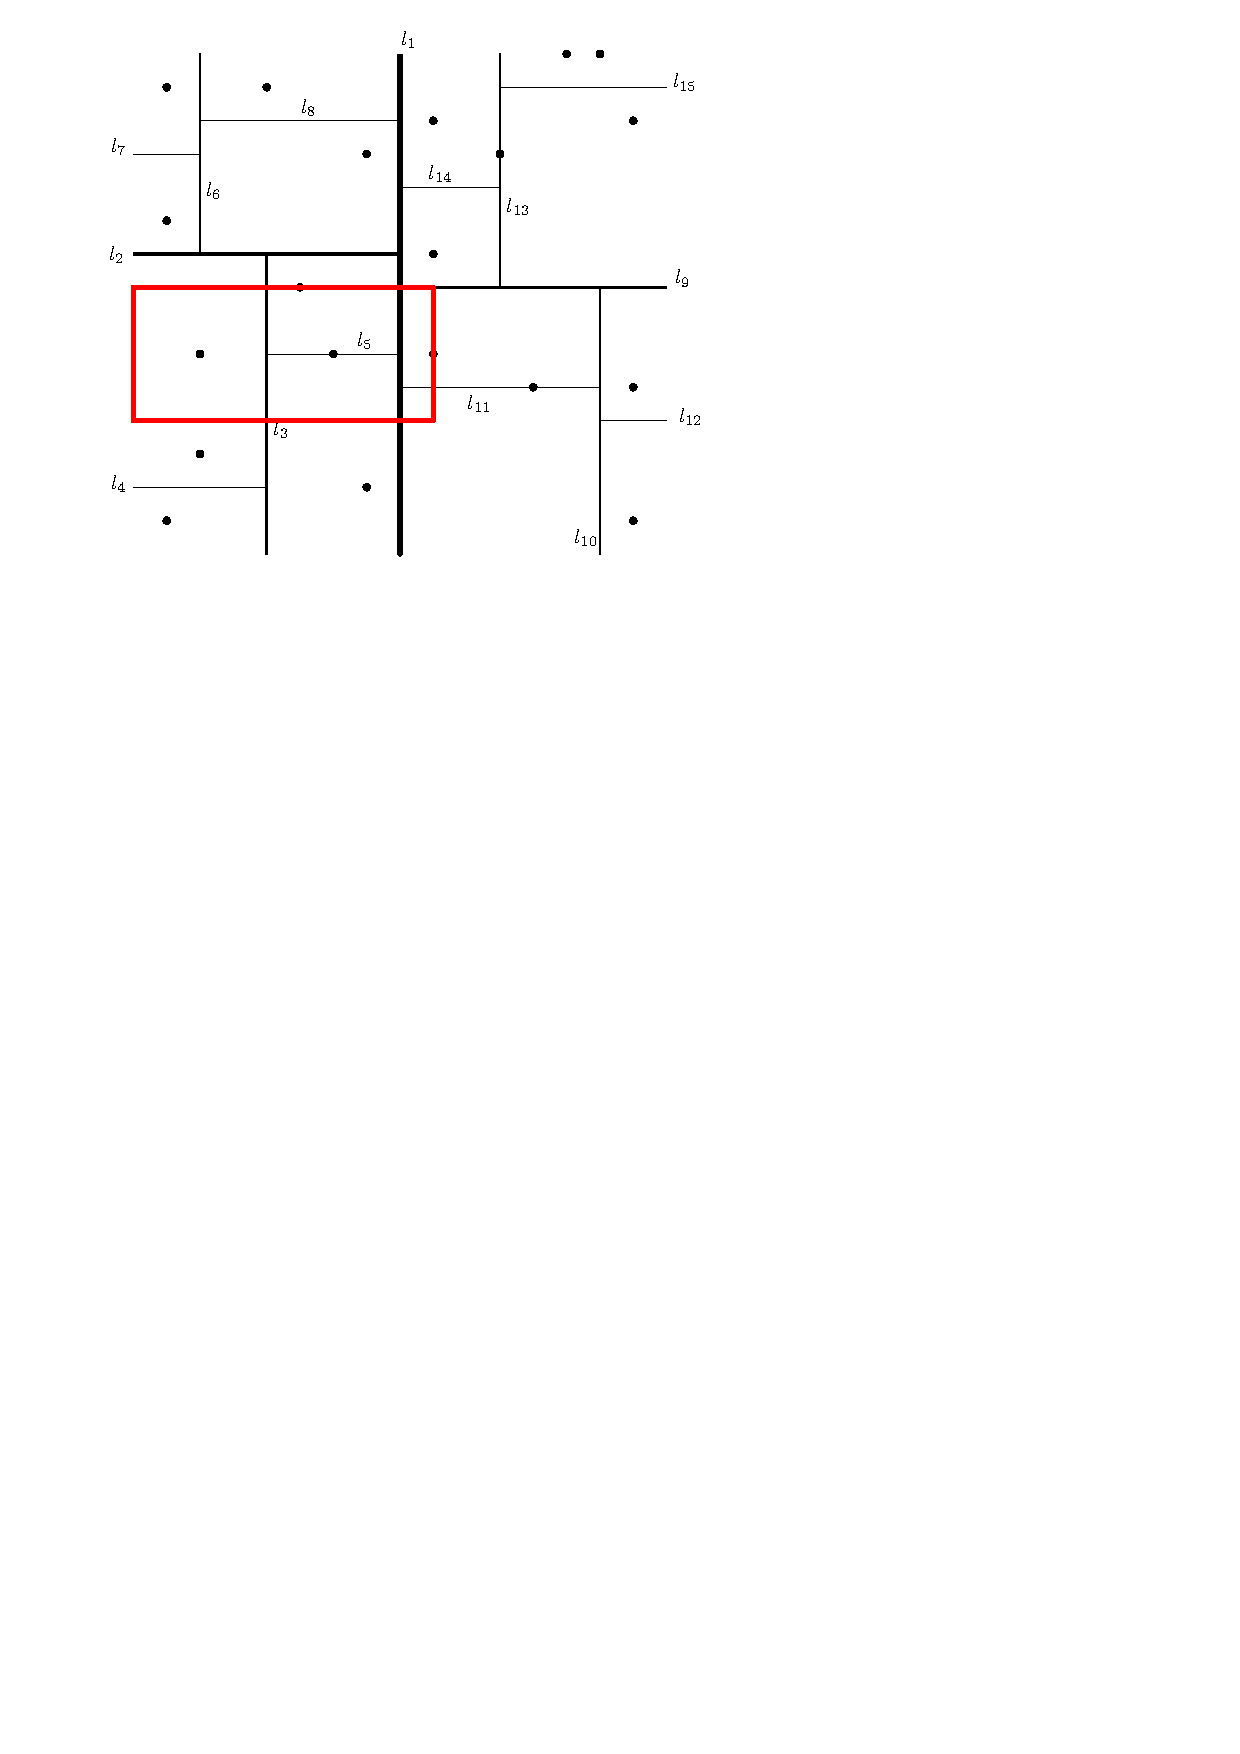
\includegraphics{figs/kdTreePlaneRectangle}
\caption{\textit{A 2D space subdivided by a KD tree, and a range query represented with a rectangle.}}
\label{figure:kdprect}
\end{figure}
In Figure \ref{figure:kdprect}, a range query is represented by a red rectangle. The question, what data points with coordinates $(x, y)$ are such that $A_x \leq x \leq B_x \land A_y \leq y\leq B_y$ is equavalent to the question: which points in the figure are in the rectangle bounded by the points $(A_x, A_y)$ and $(B_x, B_y)$. This is probably why range queries were called region queries in the original paper. The geometric interpretation of range queries works even in higher dimensions, but it gets harder to visualize. Range searches with KD trees are covered more in depth in \cite{kakde2005range}.\\
\indent Another use described in the original paper is for the nearest neighbor algorithm. They can also be used in point cloud collision detection \cite{schauer2015collision}, geographical databases \cite{ooi1987spatial}, in robotic applications \cite{cai2021ikd}, etc.

\subsubsection{Complexity}
An important paper written by Friedman et al. \cite{friedman1977algorithm} analyzes the data structure and compares it to other established data structures invented to solve similar problems. Firstly, looking at the memory complexity, we know that, in the worst case, at each depth of the tree, there are twice as many nodes as in the previous level. If we assume that the tree has $N$ leaves, the size of the tree is
\[
	\sum_{i=0}^{log_2 N}{2^i} = 2N - 1.
\]
Thus the memory complexity belongs to $O(N)$. As the number of leaves is usually proportional to the number of data points, the memory complexity will be analogous. The time complexity is calculated by solving the recurrence relation
\[
T_N = 2T_{N/2}+kN \implies T_N \in O(kN\log N).
\]
This relation works for the construction algorithm suggested in \cite{friedman1977algorithm}, in which we choose the discriminator by taking the dimension which has the largest spread in values. We will need to go over $kN$ values at each node. If this is not the case, and we take discriminators in cyclical fashion, we can just look at $N$ values to pick the splitting hyperplane, we also need to put all $N$ values into their respective child nodes, using
\[
T_N = 2T_{N/2}+N \implies T_N \in O(N\log N).
\]
This is also true if we are looking at KD trees in a specified number of dimensions (for example 3D), making the value $k$ a constant. The particular time complexities of operations on the tree depend on the implementation. The original paper by Bentley \cite{bentley1975multidimensional} claims $O(\log N)$ deletion of nodes (except the root), $O(\log N)$ insertion, and $O(N\log N)$ optimization of the tree, so the traversal can be $O(\log N)$.

\section{Surface Area Heuristic}
While the algorithm to find the splitting hyperplane can be arbitrary, in practice three of them are most well known: the spatial median, the object median and the Surface Area Heuristic (SAH). The spatial median picks the plane that splits the current space in half. The object median picks the median object along the discriminating axis and takes a plane that passes through it. The median object is usually found with an algorithm that solves for the $k$-th smallest element, with $k$ being half of the number of elements. Popular algorithms for this are PICK \cite{blum1973time}, Quickselect \cite{gibb1961algorithm} and Introselect \cite{musser1997introspective}. The SAH is a bit more complex, but it is by far the most used method. It is described in detail by McDonald and Booth \cite{macdonald1990heuristics} in 1990. They also show that the object median algorithm has the same performance as the spatial median.\\
\noindent The SAH employs two assumptions: 
\begin{itemize}
  \item All rays intersect the bounding volume represented by the root.
  \item The rays are spatially uniformly distributed.
\end{itemize}
The SAH utilizes the observation that the probability of a ray intersecting a node is equal to the surface area of the node divided by the surface area of the root. This gives us the following estimates, as stated in \cite{macdonald1990heuristics}.\\
The number of interior nodes hit per ray is
\[
	\sum_{i=1}^{N_i}{\frac{SA(i)}{SA(root)}},
\]
the number of leaves hit per ray is
\[
	\sum_{l=1}^{N_l}{\frac{SA(l)}{SA(root)}}, \text{and}
\]
the number of objects tested for intersection per ray is
\[
	\sum_{l=1}^{N_l}{\frac{SA(l)\cdot N(l)}{SA(root)}},
\]
where\\
$N_i$ is the number of interior nodes,\\
$N_l$ is the number of leaves,\\
$N(l)$ is the number of objects stored in leaf $l$,\\
$SA(i)$ is the surface area of interior node $i$, and\\
$SA(l)$ is the surface area of leaf node $l$.\\

\noindent With this, the cost of a tree can be derived as
\[
	\left( C_i \cdot \sum_{i=1}^{N_i}{SA(i)} + C_l \cdot \sum_{l=1}^{N_l}{SA(l) + C_o \cdot \sum_{l=1}^{N_l}{SA(l) \cdot N(l)}} \right) \cdot \frac{1}{SA(root)},
\]
where:\\
$C_i$ is the cost of traversing an interior node,\\
$C_l$ is the cost of traversing a leaf, and\\
$C_o$ is the cost of testing an object for intersection.\\

\noindent More importantly we can approximate the cost of splitting a node with a plane at position $b$,
\begin{equation}
	\label{eq:sah}
	f(b) = LSA(b) \cdot L(b) + RSA(b) \cdot R(b) - SA \cdot n.
\end{equation}
\noindent Where:\\
$LSA(b)$ is the surface area of left subnode,\\
$RSA(b)$ is the surface area of right subnode,\\
$L(b)$ is the number of objects to the left of the plane at $b$,\\
$R(b)$ is the number of objects to the right of the plane at $b$,\\
$n$ is the number of objects in the node, and\\
$SA$ is the surface area of the node.\\

\noindent The paper assumes no objects lie on the splitting plane, so $R(b) = n - L(b)$. In reality this will not be the case, but in practice it is most often handled in a way which either assigns the triangles to be "left" or "right" of the plane (or sometimes both), or splits them \cite{havran2002improving}. In practice, $L(b)$ and $R(b)$ are most often defined as the number of triangles assigned to the left and right child nodes, respectively, rather than the number of triangles strictly to the left or to the right of the plane. Nonetheless, we chose to leave the original definition for accuracy. A more common practical definition along the lines of \cite{wald2006building} would be\\
\begin{equation}
	\label{eq:tsah}
	Cost = C_i + C_o \left(\frac{SA(left child)}{SA(node)}|T_L| + \frac{SA(right child)}{SA(node)}|T_R| \right),
\end{equation}
\noindent where:\\
$|T_L|$ is the number of triangles assigned to left child, and\\
$|T_R|$ is number of triangles assigned to right child.\\

\noindent The equation for splitting the node, \eqref{eq:sah} or \eqref{eq:tsah}, is the crux of the heuristic, we want to minimize its value at every node.\footnote{The $(SA - n)$ part of \eqref{eq:sah} is usually omitted, as we can see in \eqref{eq:tsah}, since it does not depend on the position of the splitting plane $b$. It can, however, be used to determine whether to split the node at all.} Finding or approximating the minimum of this function efficiently is the biggest focus of a lot of scientific studies of KD trees in the context of ray tracing, since finding the tree which has the lowest total cost is infeasible due to the number of possible trees.\\
\indent An important observation to make is that for some interval $\left(x, y\right)$ and $p \in \left(p_x, p_y\right)$ where $|T_L|$ and $|T_R|$ do not change, the $Cost$ function changes linearly. So we would only need to check the value of the function at $x$ and $y$ to find its minimum on that range. Therefore, it is enough to check $Cost$ only at the points where $|T_L|$ and $|T_R|$ change to find its minimum \cite{wald2006building}. We now have finitely many split candidates we need to check, as opposed to an infinite amount of continuous values.\\
\indent Additionally, the function $f(b)$ from \eqref{eq:sah} and the $Cost$ from \eqref{eq:tsah} are approximations of the actual cost of splitting the node at the plane, since they do not take into account the fact that the child nodes may be split further, which would reduce their actual cost. The exact function would be recursive and it would yield an optimal tree, but it would comparatively be very slow.\\
\indent Another observation can be made by taking the first derivative of the function $f(b)$. The plane which minimizes the surface area heuristic must lay between the planes for the object median (when $L(b) = \frac{n}{2}$) and spatial median (when $LSA(b) = RSA(b)$) \cite{macdonald1990heuristics}. This can limit the range in which we need to look for the minimum considerably.

\section{Exact SAH in $O(N\log N)$}
One of the famous papers in regard to KD trees with ray tracing was written by Wald and Havran \cite{wald2006building} in 2006. It proposes an algorithm for building good KD trees for ray tracing using SAH and in $O(N\log N)$ complexity -- the theoretical lower bound. In order to describe the algorithm we first need to understand the notation used.\\
\indent The space (voxel) represented by a node is denoted with $V$. The spaces represented by the nodes children are $V_L$ for the left child and $V_R$ for the right child. $T$ is the set of all triangles represented by a node. $T_L$ is the set of all triangles in $V_L$ that do not intersect the splitting plane $p$. Similarly, $T_R$ is the set of all triangles in $V_R$ that do not intersect $p$. All triangles in $T$ that intersect $p$ are in $T_P$. $N$ is the number of triangles in the current node, thus $N=|T|$. Similarly, $N_L$ is the number of triangles that belong to the left child, and $N_R$ is the number of triangles that belong to the right child.\\
\indent The first thing to note about the algorithm is the use of split clipping introduced in a paper by Havran and Bittner \cite{havran2002improving}. Since the SAH can only be minimal when $|T_L|$ and $|T_R|$, i.e. $N_l$ and $N_r$, change, it is sufficient to use the AABBs of the triangles as split candidates. This implies 6 planes for each triangle. We can however run into trouble with this method, if an AABB of a triangle belongs to a voxel even though the triangle does not intersect it (as in Figure \ref{figure:sc1}) or a plane we have chosen intersects an AABB but it does not intersect the triangle (as in Figure \ref{figure:sc2}). To solve this, we will only looked at the triangles after clipping them to the voxel i.e. for each triangle $t$ we will take for the split candidates the six planes determined by $\mathcal{B}(t\cap V)$.\\
\indent To solve triangles overlapping the plane, we will calculate the SAH for the scenario that we put $T_P$ in $T_L$ and in $T_R$ and do the one with the smaller cost. This way no triangle belongs to two nodes, which means there will not be any extra checks. This is not the only way to achieve this, as mentioned in \cite{havran2002improving}, but gives best results in practice.
\begin{figure}
\centering
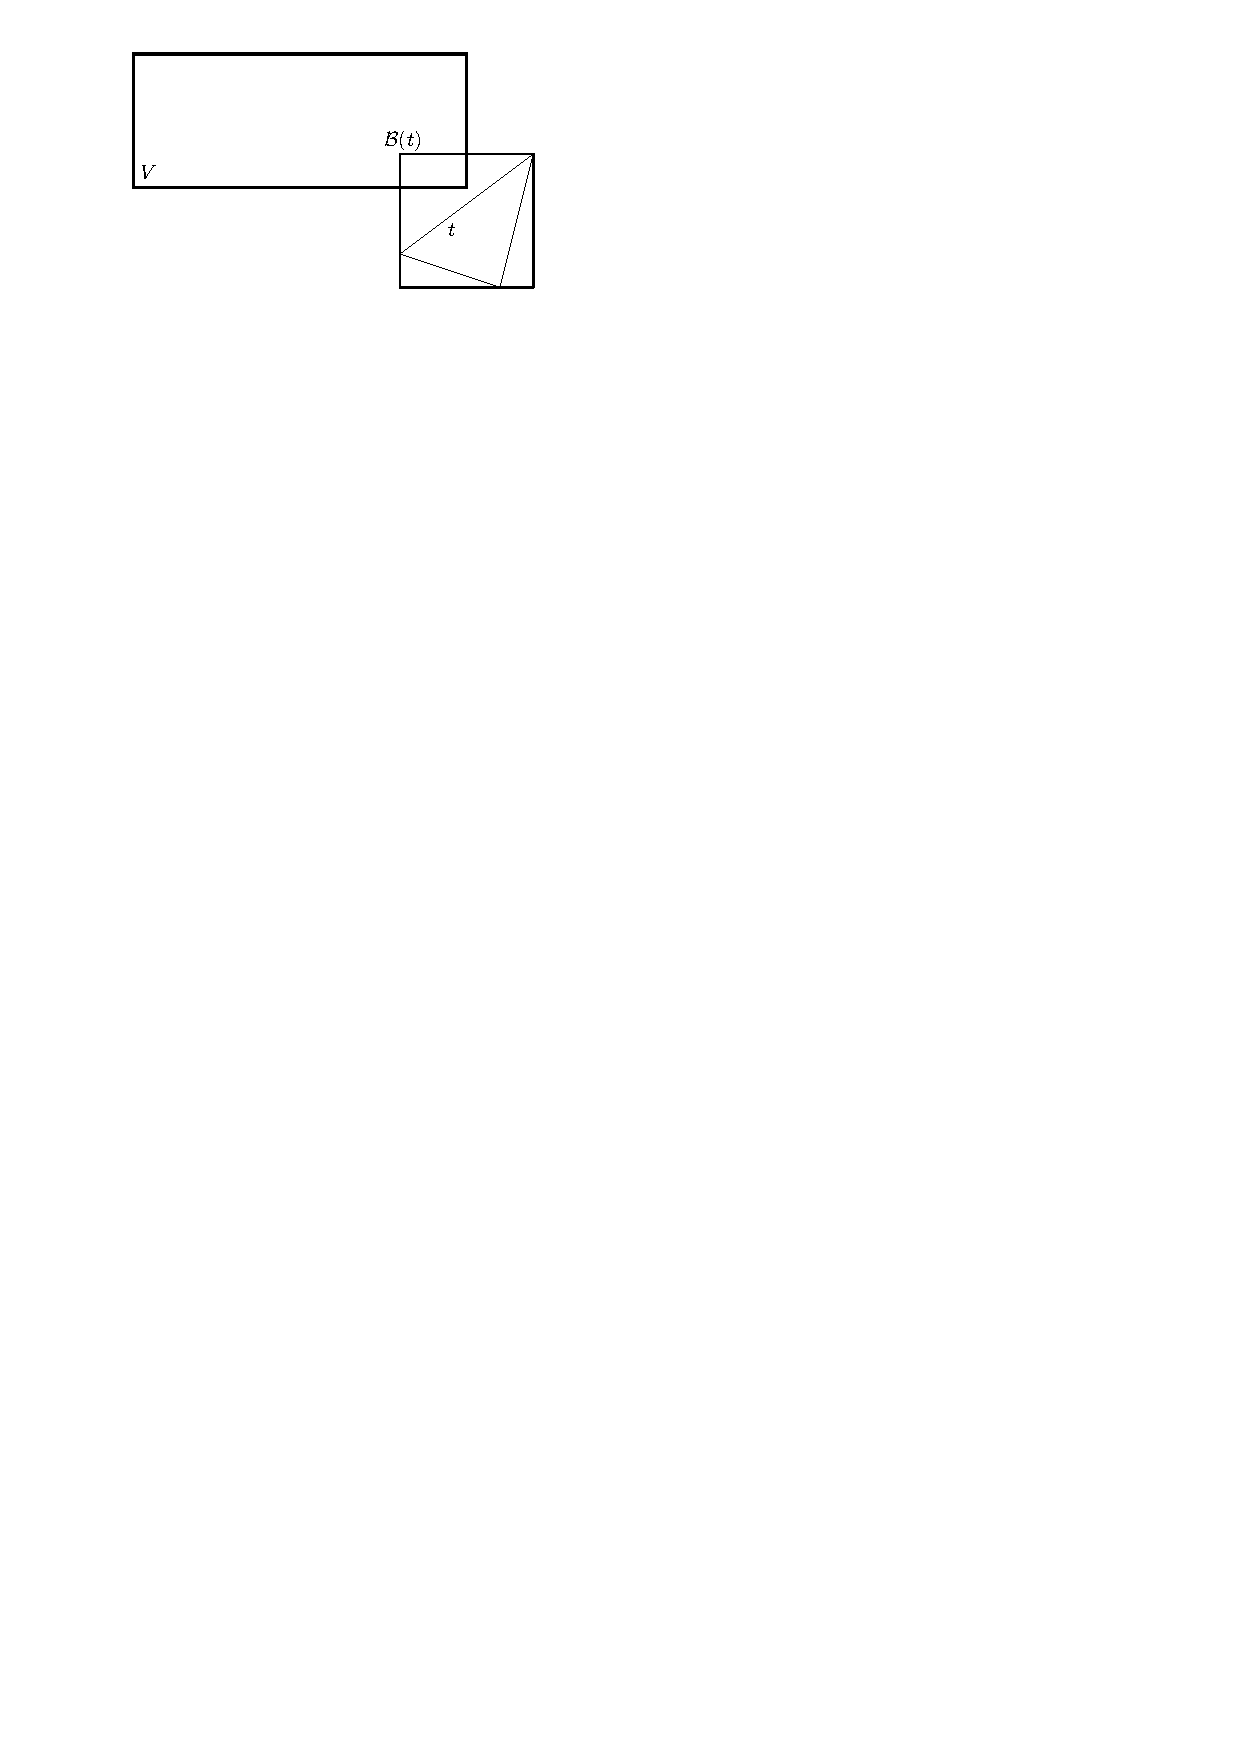
\includegraphics{figs/splitClipping1}
\caption{\textit{$\mathcal{B}(t)$ overlaps $V$ but the triangle $t$ does not.}}
\label{figure:sc1}
\end{figure}
\begin{figure}
\centering
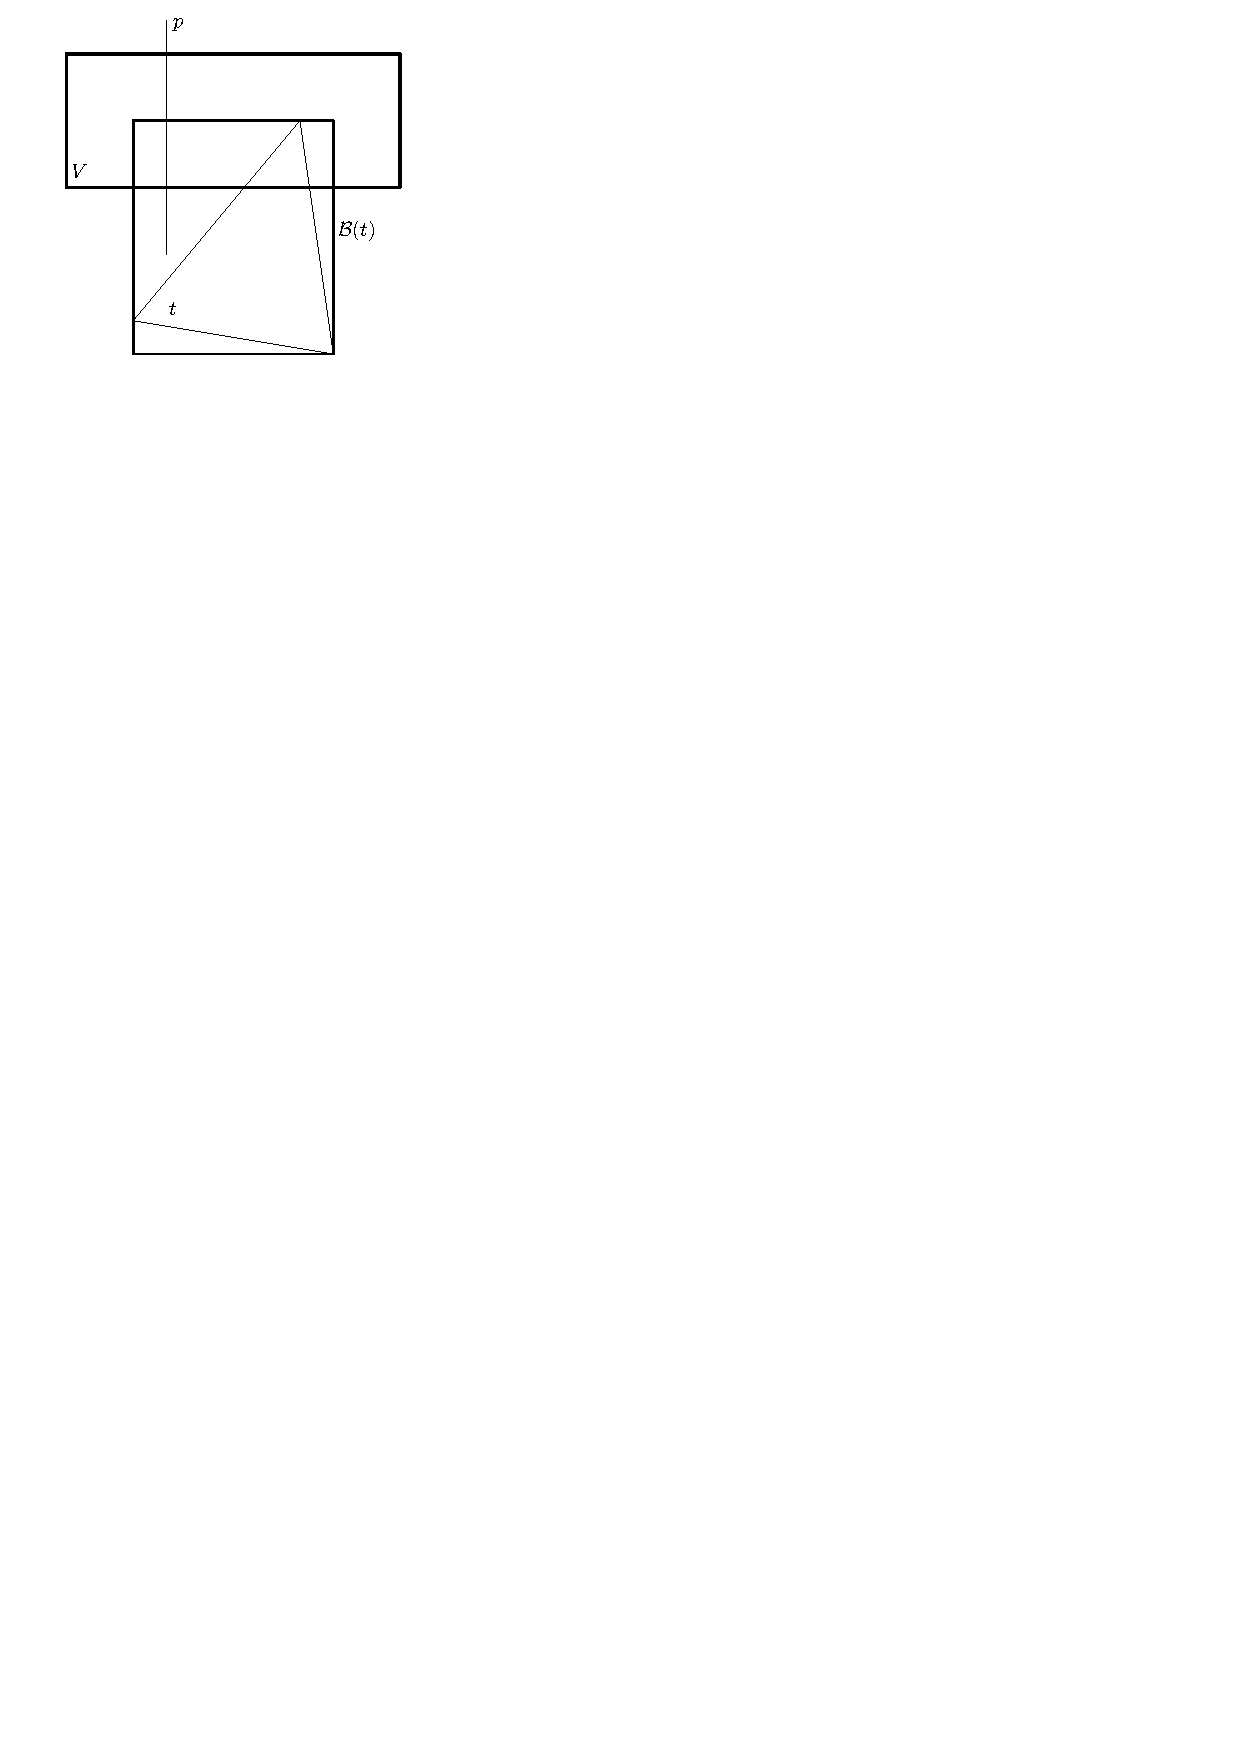
\includegraphics{figs/splitClipping2}
\caption{\textit{The splitting plane $p$ intersects $\mathcal{B}(t)$ but does not intersect the part of the triangle inside $V$.}}
\label{figure:sc2}
\end{figure}
\begin{figure}
\centering
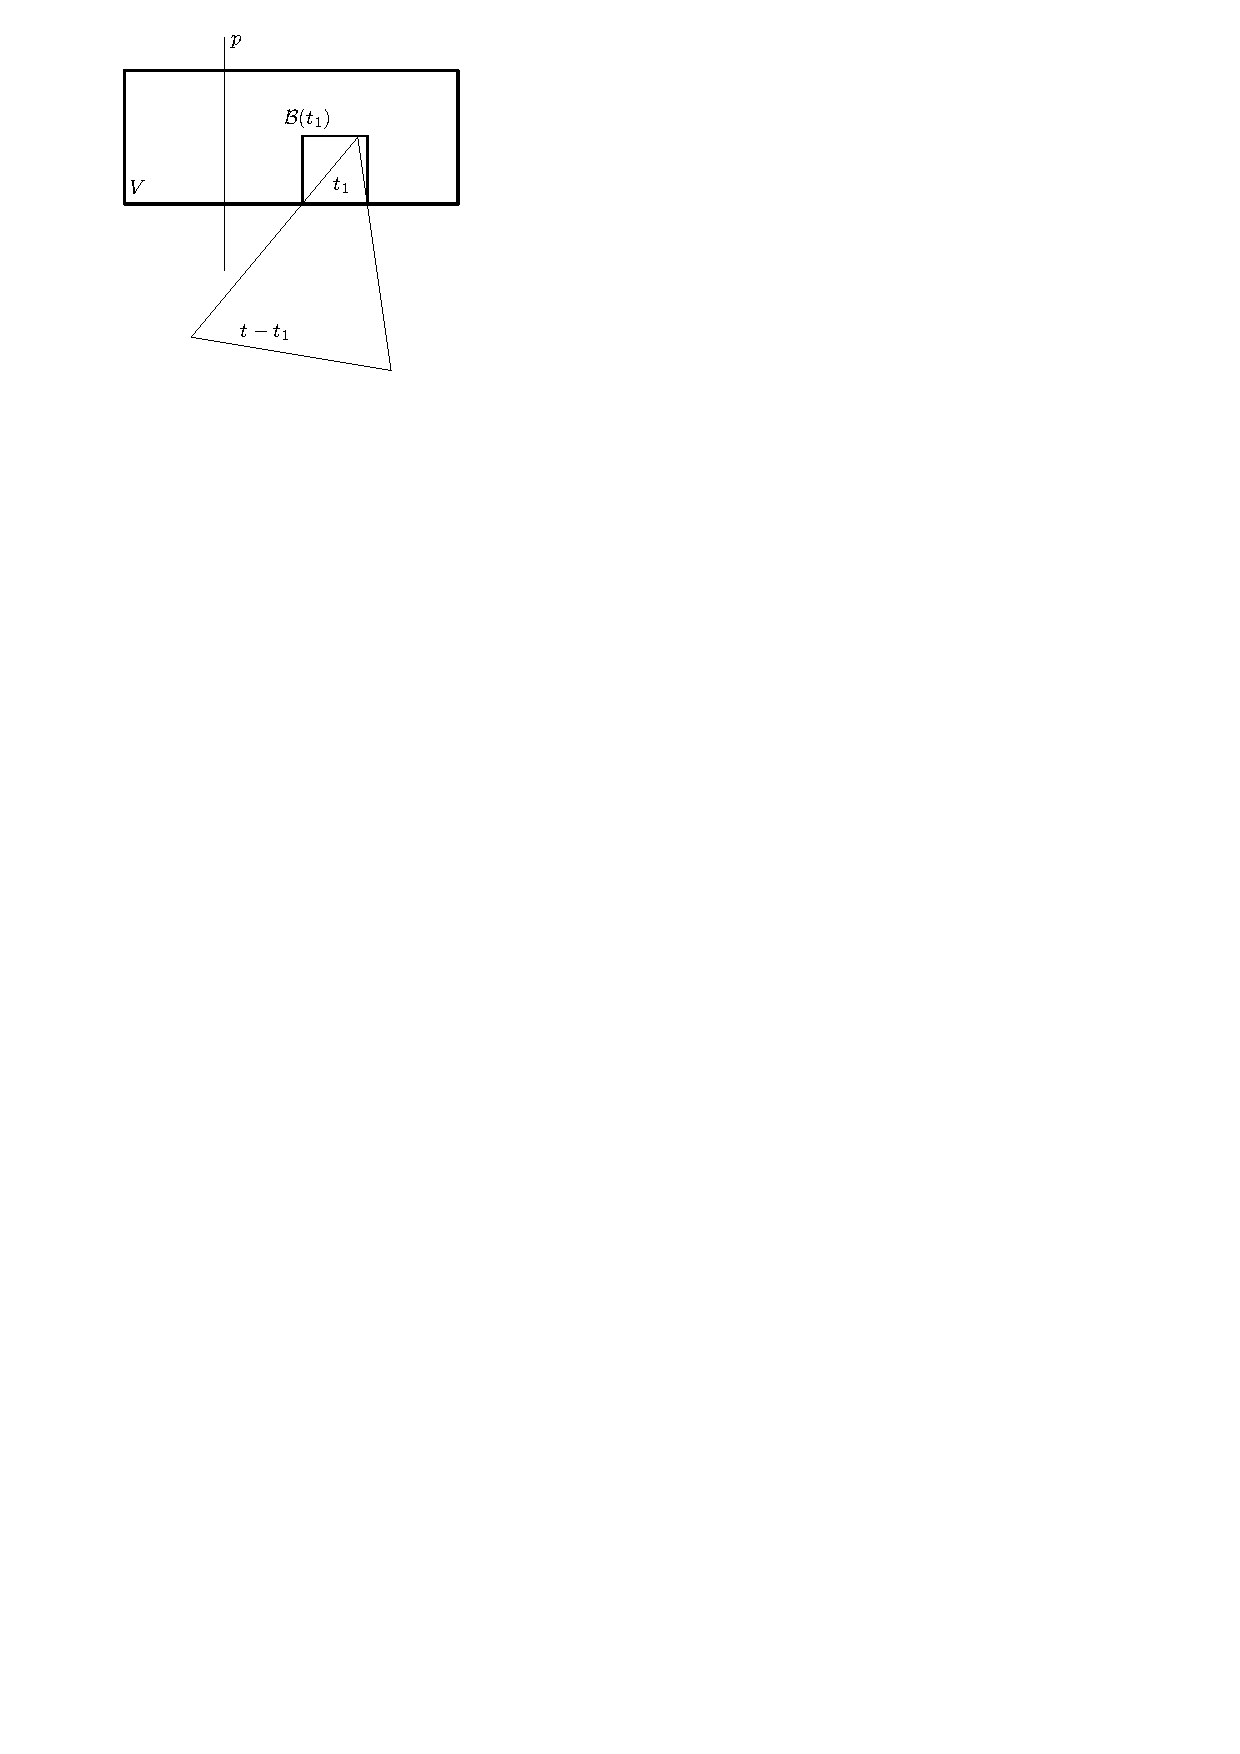
\includegraphics{figs/splitClipping3}
\caption{\textit{We clip $t$ to $V$ so now we have accurate information. $\mathcal{B}(t_1)$ does not intersect the plane. We can easily triangulate $t-t_1$ and give it to the neighboring voxel.}}
\label{figure:sc3}
\end{figure}

\indent Now we can easily calculate the surface area heuristic for each split in $O(1)$, and we can go over all split candidates in $O(N)$ since there is a maximum of $6N$ splits. The only problem left is to connect those two; we need a way to efficiently calculate $N_L$, $N_R$ and $N_P$ to calculate the SAH for a particular split. For this, a line sweep algorithm is used. Lets, for some plane $p$, define $p^+$, $p^-$ and $p^|$ as the number of triangles starting, ending and lying completely on the plane. Now if we fix a dimension, and sort all planes in that dimension increasingly we can go over them from left to right and calculate $N_L$, $N_R$ and $N_P$ like this:
\begin{align*}
& N_L^{(i)} = N_L^{(i-1)} + p_{i-1}^| + p_{i-1}^+\\
& N_R^{(i)} = N_R^{(i-1)} - p_i^| - p_i^-\\
& N_P^{(i)} = p_{i}^|
\end{align*}
\noindent We can see the visualization of the algorithm with Figures \ref{figure:sweep1} and \ref{figure:sweep2}. The implementation of this algorithm is not that complicated. For each triangle, we generate a "planar event" if the triangle is parallel to the plane that is going to be sweeping, otherwise we generate a "start event" and an "end event". These events will have a referance to their triangle, the corresponding plane, and their type. We can sort these events by the position of their plane. If two events have the same position we compare their types, where end event $<$ planar event $<$ start event. We go over these events one by one, and keep updating $N_L, N_R, N_P, p^+, p^-, p^|$ and calculating SAH for each split candidate. The number of events for an axis belongs to $O(N)$.
\begin{figure}
\centering
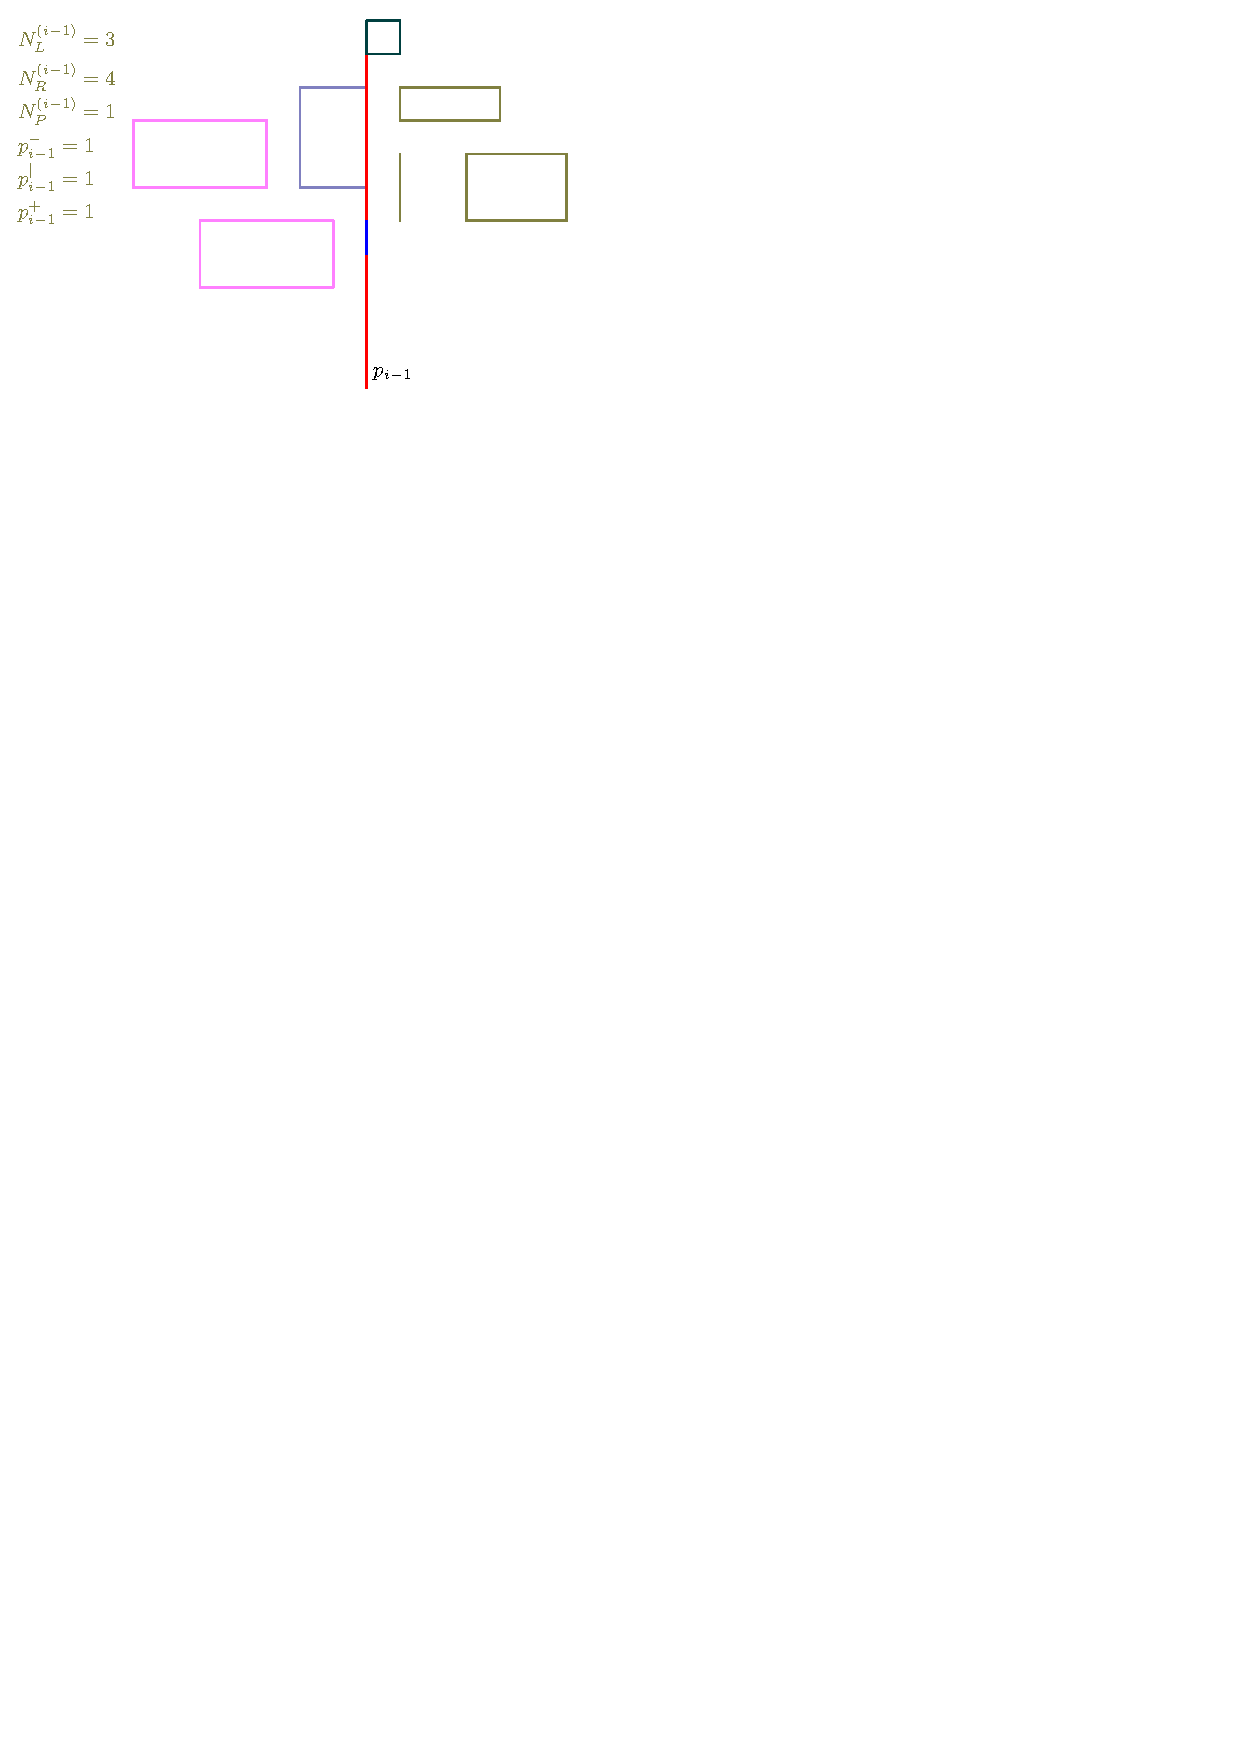
\includegraphics{figs/sweep1}
\caption{\textit{Sweep algorithm at step $i-1$. Triangles are represented by their AABBs, two of them are parallel to the plane.}}
\label{figure:sweep1}
\end{figure}
\begin{figure}
\centering
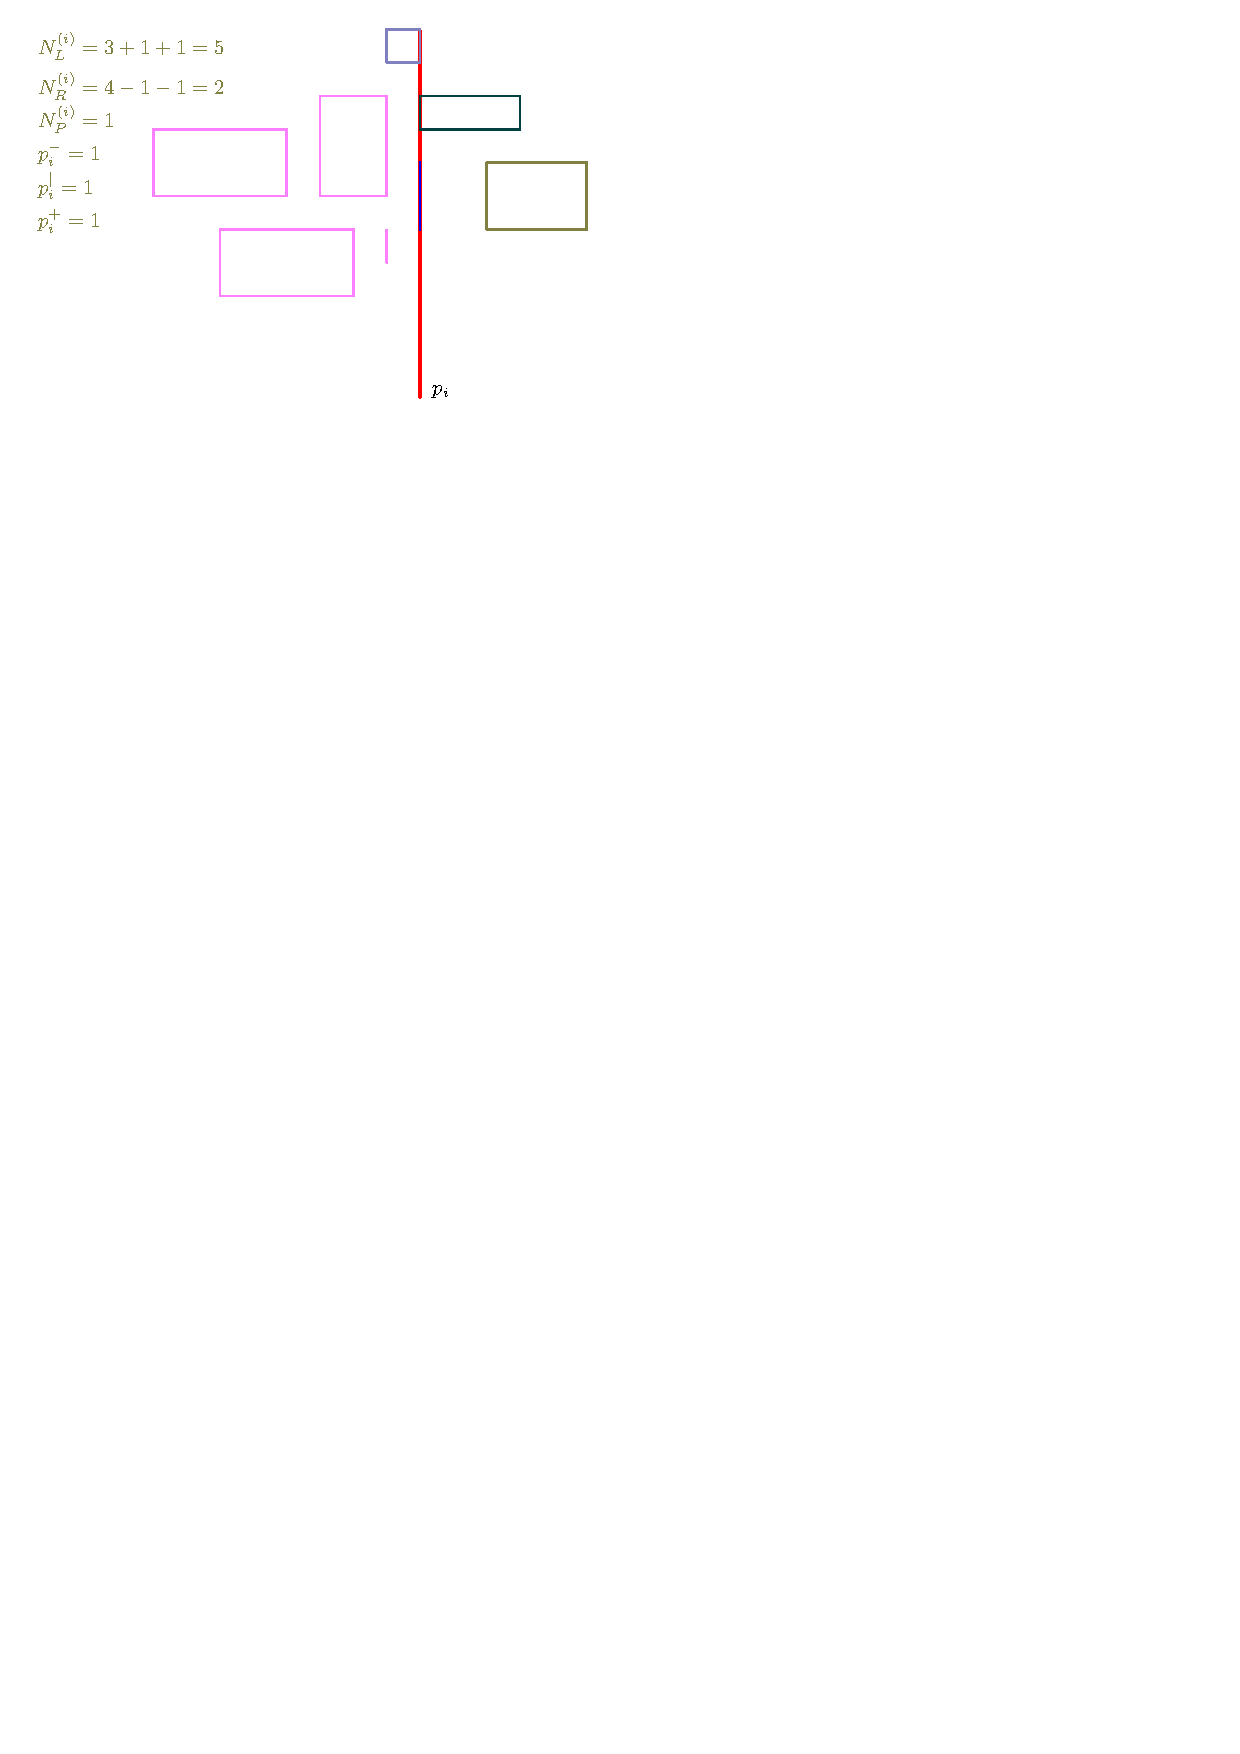
\includegraphics{figs/sweep2}
\caption{\textit{Sweep algorithm at step $i$, with values updated according to the algorithm.}}
\label{figure:sweep2}
\end{figure}

\indent Currently we have $T(N) = 2T(N/2) + N\log N$ which is $O(N\log^2N)$. The square factor is coming from the fact that we are sorting the events in every node ($O(N\log N)$ operations), to achieve the theoretical lower bound of $O(N\log N)$ we need to perform at most $O(N)$ operations in each node. This is done by pre-sorting the events and keeping them sorted for every node during the construction of the tree. Pre-sorting the events ($E$) is not a problem, we just have to additionally keep track of their dimensions. Keeping them sorted for every node is more complicated and described in 4 steps:\\
\indent \textbf{Step 1:} Classification: After finding the plane $p$ in a node, we need to figure out where each triangle is going to go: $T_L$ or $T_R$. $T_P$ is already determined to belong to one of those. For triangles that do not overlap $p$ we can easily determine this by iterating over the sorted events list and comparing the event positions to the position of the plane $p$. Every event has an assosiated triangle so non-overlapping triangles can be easily classified.\\
\indent \textbf{Step 2:} Splicing $E$ into $E_{LO}$ and $E_{RO}$: We iterate over all the events and put events that belong to left only triangles in $E_{LO}$ which will go only to the left child node, and we put right only triangle events in $E_{RO}$ which will go only to the right child node. Note that both $E_{LO}$ and $E_{RO}$ are sorted.\\
\indent \textbf{Step 3:} Generating $E_{BL}$ and $E_{BR}$ for triangles overlapping $p$: We clip the triangles overlapping $p$ to $V_L$ and $V_R$ and put the generated events in $E_{BL}$ and $E_{BR}$ respectively. $E_{BL}$ and $E_{BR}$ are not sorted.\\
\indent \textbf{Step 4:} Merging the four strains: All of the events belonging to $E_L$ are compromised of the elements in $E_{LO}$ and $E_{BL}$. Similarly $E_R$ is going to be comprosised of $E_{RO}$ and $E_{BR}$. If we sort $E_{BL}$ and $E_{BR}$ we can merge them with $E_{LO}$ and $E_{RO}$ respectively in $O(N)$ time, using the merging technique from mergesort. If we assume that only $O(\sqrt{N})$ triangles overlap $p$, sorting the arrays will be $O(|E_{BL}|\log |E_{BL}| + |E_{BR}|\log |E_{BR}|) = O(\sqrt{N}\log \sqrt{N})\subset O(\sqrt{N}\times \sqrt{N}) = O(N)$. This is enough to achieve a total time complexity of $O(N\log N)$.\\
\indent The assumption that no more than $O(\sqrt{N})$ triangles intersect a given plane is cited to hold for reasonable scenes \cite{de2002realistic}. This is the only assumption made necessary for the complexity of the algorithm. In the worst possible case of the number of triangles intersecting the plane being $O(N)$, the sorting of $E_{BL}$ and $E_{BR}$ will take $O(N\log N)$ and the total algorithm time complexity will be $O(N\log^2N)$ - still very performative.\\
\begin{table}
\centering
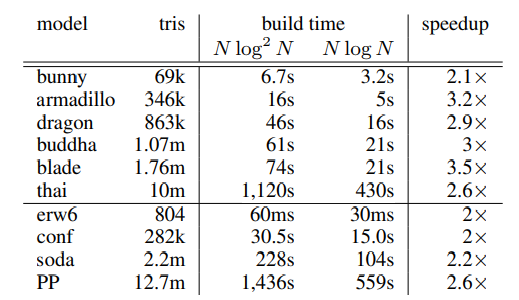
\includegraphics{figs/nlognTable}
\caption{\textit{This is the table for comparison of the known $O(N\log^2N)$ and new $O(N\log N)$ algorithm. \cite[Table 2]{wald2006building}.}}
\label{table:nlogn}
\end{table}
\indent A great feature of this algorithm is its well-defined time complexity. Many methods for contsructing KD trees have been invented and for many of them it is very hard or impossible to calculate a useful time complexity. Thus, these algorithms are usually compared by benchmarking their times. This, however, can be rather inconsistent since it can depend on some low level optimizations, the computer architecture, and the particular scene being used. With algorithms with well defined time complexities, we can easily compare them and guarantee their performance across all architectures and scenes. It is also important to mention that the time complexity for this particular algorithm meets the theoretical lower bound. Thus, any algorithms that perform faster will need to find a way to approximate the minimum for the SAH, while here it is calculated exactly. Nonetheless, although the SAH function is minimized at each node, that does not mean that the algorithm produces an optimal tree, so there are possible improvements there. We can also see in Table \ref{table:nlogn} that, unexpectedly, the speedup of the algorithm as compared to $O(N\log^2N)$ does not necessarily increase, with an increased number of triangles, which is sligthly dissapointing.

\section{An Adaptive Error-Bounded Heuristic}
As previously stated, optimized KD trees, which calculate the exact minimal SAH for each node, are impractical if we require faster performance. This is, for example, a big problem in dynamic scenes where the tree needs to be rebuilt every frame. One tree building algoritm which approximates the SAH, and performs faster than the algorithm by Wald and Havran \cite{wald2006building} was presented in a paper by Hunt et al. in 2006 \cite{hunt2006fast}.\\
\indent The algorithm described does not use sorting, but rather "scanning". In the sorting approach we calculate the SAH for all triangles, or rather their AABBs events, from left to right while keeping track of how many triangles there are to the left and to the right of the current plane. In the scanning approach for every plane for which we want to perform the heuristic we have to go over all the AABBs to determine which are to the right and which are to the left of the plane. So an unoptimized sorting approach performs $O(N)$ SAH calculations in $O(N \log N)$ in a single node. We have already seen how this can be optimized. The scanning approach performs $q$ queries in $O(Nq)$ which looks significantly worse. If we fix $q$ as a constant, which is equal to eight in the paper, the tree with the scanning approach will be built in $O(N\log N)$ which is the same as the algorithm by Wald and Havran \cite{wald2006building} except with way less checks for the SAH. It would seem that the scanning approach is objectively worse, but in reality this is not the case. The algorithm in the paper performs significantly faster than the sorting $O(N\log N)$ one, while producing only slightly worse trees. Note that the whole point of the existence of the tree is to allow us to perform faster ray tracing, so the time spent constructing the tree cannot be overlooked. The general layout of the proposed algorithm is as follows:
\begin{itemize}
\item We first uniformly sample the SAH. We can do this since our planes do not need to be determined by the AABBs when scanning. In the paper the function is sampled at 8 points.
\item Then we sample the function again at the intervals which we learned are particularly unpredictable from the previous step. In the paper this makes an additional 8 points.
\item We than interpolate this function using piecewise-quadratic interpolation, i.e. we stitch together quadratic approximations of the function between every two points.
\item We easily find the minimum of this interpolated function, since it is just the minimum of many quadratic functions which are easy to calculate, and take that as the approximation of the minimum of the SAH.
\item We split the triangles to ones left and right of the plane representing the approximated minimum SAH, and recurse to the child nodes.
\end{itemize}
\indent Lets explain this further. In reality the actual cost function is not directly interpolated quadratically, but its inputs are interpolated linearly, and from that, a piecewise-quadratic approximation for the heuristic is calculated. The inputs are the cost of the left child, the cost of the right child, the surface area to the left of the plane and the surface area to the right of the plane. These are written as $C_L$, $C_R$, $SA_L$ and $SA_R$ in the paper. $C_L$ and $C_R$ are approximated to be the number of AABBs overlapping the left and right child respectively. \\
\indent Throughout the paper the function $C_L - C_R$ is used instead of the SAH cost function since the bounds on it bound both $C_L$ and $C_R$ and thus bound the cost function. The function $C_L(x) - C_R(x)$ is nondecreasing. To adaptively choose the second set of points, we want to put more points on the intervals where there is a greater change in the function. Since the function is nondecreasing this can be done by placing the new $q$ points uniformly along the range of $C_L - C_R$, the values of the function. After uniformly placing the sample points we assign each of them the interval they belong to, and then we uniformly distribute the points inside each interval. This can be seen in Figures 3 and 4 in the paper, presented here as Figures \ref{figure:samp1} and \ref{figure:samp2}. The product of cost error and position error between adjacent pairs of samples is bounded by $O(1/q^2)$ as proven in the papers Appendix A. A comparison between the approximate functions and their actual graph is given with Figures 5 and 6 in the original paper, presented as Figures \ref{figure:ac} and \ref{figure:tc} here. It is also noted in the paper that for deep nodes a switch to exact SAH evaluation should be made. This is because for deep nodes the cost function is much less smooth so the approximation is more prone to error. They classified "deep" nodes as those containing 36 AABBs or less. Also, using the approximate algorithm as opposed to brute-force checking for such a small number of AABBs does not yield to a noticable performance decrease. Reportedly, in practice, the exact scanning $O(N^2)$ method is preferable to the exact $O(N\log N)$ one for such small $N$, where $N$ is the number of AABBs. \\
\indent Finally, the researhers propose three variants of the algorithm based on how we choose the discriminator:\\
- one axis - evaluate along just the longest axis\\
- hybrid - use one axis for more than some number of AABBs (they used 1024), use all axes otherwise\\
- all axes - evaluate on all axes\\
\indent In reality, a lot of the focus on ray tracing is in the context of dynamic scenes, and as such the total time to image, composed of the tree construction time and intersection testing (rendering time), must be considered, since it needs to be performed every frame. This is especially true if we are trying to achieve real time ray tracing. This algorithm by Hunt et al. \cite{hunt2006fast} is a significant step in the right direction. Time comparisons can be seen in Tables \ref{table:12comp} and \ref{table:reninc}. Furthermore, this algorithm delegates a lot of the work to the deeper parts of the tree, so it sees a big performance improvement if lazy building is utilized as Hunt et al. have demonstrated in 2007 \cite{hunt2007fast}. Lazy building will become integral for dynamic scenes since it will allow us to not need to rebuild the whole tree every frame \cite{shevtsov2007highly}. It is important to note that the methods described here are not exclusive to KD trees and can be extended to BVHs, a big contender for acceleration structures. Also, importantly, the switch from sorting to scanning allows us to perform several computations in parallel, which was not possible when the order of execution was important. More and more algorithms for raytracing are focusing on the actual implementation and connection with the hardware. This is becoming more important, as hardware tailored for ray tracing is being produced. The algorithms will need to take it into account, along with an increased focus towards parallel processing.
\begin{figure}
\centering
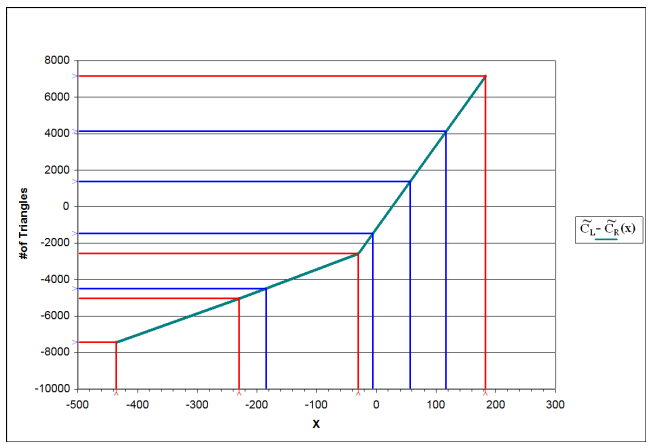
\includegraphics[width=12cm]{figs/sampling1}
\caption{\textit{Red lines indicate the initial $q$ samples. Blue lines indicate the evenly spaced new $q$ samples for determining their intervals. \cite[Figure 3]{hunt2006fast}.}}
\label{figure:samp1}
\end{figure}
\begin{figure}
\centering
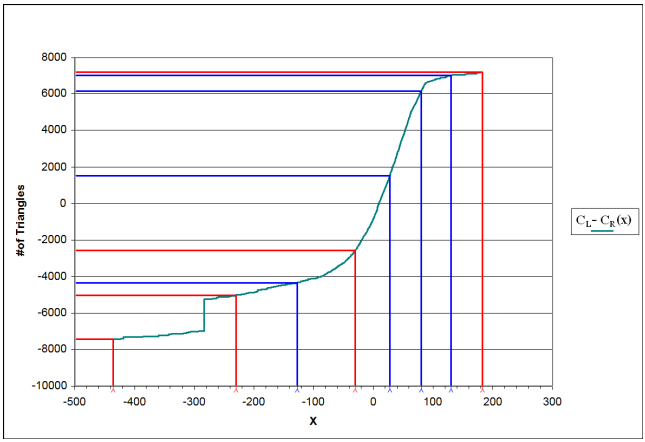
\includegraphics[width=12cm]{figs/sampling2}
\caption{\textit{The blue lines indicate the new $q$ blue samples after they are distributed within their intervals. \cite[Figure 4]{hunt2006fast}. }}
\label{figure:samp2}
\end{figure}
\begin{figure}
\centering
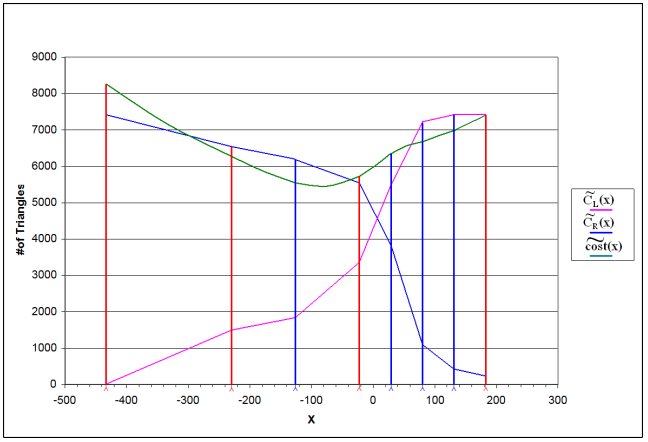
\includegraphics[width=12cm]{figs/approximateCost}
\caption{\textit{"Approximate $C_L$, $C_R$ and $cost$". \cite[Figure 5]{hunt2006fast}.}}
\label{figure:ac}
\end{figure}
\begin{figure}
\centering
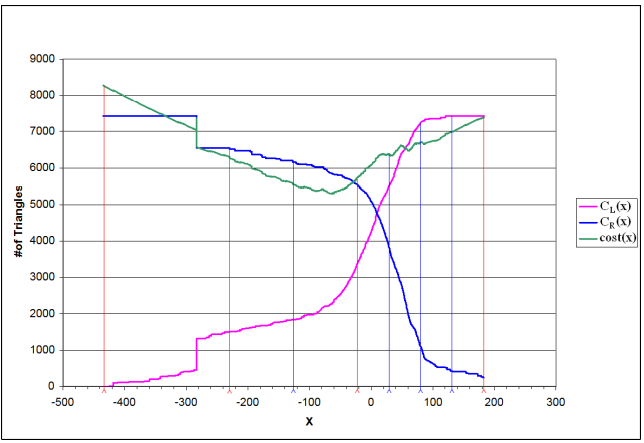
\includegraphics[width=12cm]{figs/trueCost}
\caption{\textit{The graphs of the functions $C_L$, $C_R$ and $cost$. \cite[Figure 6]{hunt2006fast}.}}
\label{figure:tc}
\end{figure}
\begin{table}
\centering
\begin{tabular}{|l|l|l|l|l|}
\toprule
Scene & All Axes (Hunt) & Hybrid (Hunt) & One Axis (Hunt) & (Wald)\\
\midrule
Bunny & 0.25 & 0.23 & 0.11 & 3.2\\
Armadillo & 1.41 & 1.14 & 0.69 & 5\\
\bottomrule
\end{tabular}
\caption{\textit{Build time of the tree in seconds. Three variations of the algorithm by Hunt et al. \cite{hunt2006fast} and the $O(N\log N)$ build by Wald and Havran \cite{wald2006building}, times taken from their papers.}}
\label{table:12comp}
\end{table}
\begin{table}
\centering
\begin{tabular}{|l|l|l|l|l|}
\toprule
Scene & All Axes (Hunt) & Hybrid (Hunt) & One Axis (Hunt) & (Wald)\\
\midrule
Bunny & 1.63\%  & 1.63\% & 7.72\% & 0\% \\
\bottomrule
\end{tabular}
\caption{\textit{The increase in rendering time (ray intersection testing). Times taken from \cite{hunt2006fast}.}}
\label{table:reninc}
\end{table}

\section{Parallel KD trees for dynamic scenes}
As the need for ray tracing in dynamic scenes, and the orientation towards parallelism intensifies, the algorithms for them keep improving. One such algorithm was written by Shevtsov et al. in 2007 \cite{shevtsov2007highly}. Particularly, it approximates the SAH using their min-max binning algorithm, allows for the parallel construction of KD trees, and has smart memory allocation which will not be covered here.\\
\indent Lets first explain how the SAH is calculated. For each node we will keep track of two arrays of bins for each dimension. One array will save the information about where each primitive (triangle AABBs) starts, the other where they end. All the bins will just be counters, counting how many primitives start / end with that particular bin. The bins span the continuous space from the start of the leftmost primitive to the end of the rightmost one. We will fill them by iterating once over the primitives, and for each primitive we will increase the counter at the bin (in the first array) at the beginning of the primitive, and increase the counter at the bin (in the second array) at the end of the primitive. This can be seen in Figure \ref{fig:binning}. The split candidates will be the bin boundaries. The number of primitives to the left of a plane will be the sum of the values in the first array (of primitive starts) up to the corresponding bin boundary. The number of primitives to the right of the plane will be the sum of the values from the corresponding bin boundary in the second array (of primitive ends) to the last bin. The surface areas are again trivial to compute. To calculate the parameters for a single boundary takes $O(N_b)$ where $N_b$ is the number of bins. We can, however, go over all the bin boundaries from left to right and keep track of the number of primitives to the left and right of the boundary trivially. Giving us the values for $N_b + 1$ split candidates in $O(N_b)$. It should be noted that some primitives will be counted to be both "left" and "right" of the splitting plane. When a boundary with the minimal SAH is found, a final pass through the primitives is done to sort them into the left and right child nodes. Similarly to the previous algorithm by Hunt et al. \cite{hunt2006fast}, we start performing exact SAH calculations at deep levels, in particular, when the number of primitives meets the number of bins. As for the value of $N_b$, their experiments have shown that 32 bins for each level of the tree is a sufficiant number. The only exception is during the decomposition phase covered below.\\
\indent An important part of the binning is that we will not in actuality go over all the triangles when constructing the bins. We will only consider every $l$-th primitive, thus just approximating the SAH cost function. In the paper a practical value of $l = log_{10}N$ is found, where $N$ is the number of primitives in the current node. This speeds up the tree construction considerably.\\
\indent Parallelizing the binning is possible, and very affective, as long as each thread is given a mutually exclusive and equal in size set of primitives. We also have the option of parallelizing building the tree, making every thread work on its own subtree. To do this we first need to divide the scene so that each thread has its own subtree. We will do this by performing parallelized binning on the whole scene. We then split the scene in two at the boundary of the bin corresponding to the median value. Each of the two children of the scene now owns half the threads. We continue the splitting recursively until the number of threads is equal to the number of sub-domains. We will need $log_2T$ decomposition levels where $T$ is the number of threads. The decomposition process can be seen in Figure \ref{fig:decomp}. It has been practically shown that for the decompositioning, using $512\cdot T$ bins is sufficient, where each decomposition node has its own $T$.\\
\indent As already mentioned the need for algorithms that perform well on dynamic scenes and are able to be easily parallelized is increasing, and this algorithm pushed the boundaries even further. Each of its components can be used seperately in combination with other algorithms, to give us better performance. The parallelization scheme is essentially applicable with any KD tree, although the decomposition will be slower for algorithms that cannot be parallelized inside of a node. Another idea mentioned in the paper is the fact that we can split the objects into those that are going to be static and those that are going to be dynamic, and build two seperate KD trees, one for static objects and one for dynamic objects, which leads to a great practical performance increase. The algorithm's approximation of the SAH is very aggresive, and although the tree quality suffers a bit and we have an increased rendering time, the construction time is reduced immensly leading to a reduction in the "time to image" \cite{shevtsov2007highly}. The time comparisons with the Wald and Havran $O(N\log N)$ can be seen in Table \ref{table:13comp}.
\begin{figure}
\centering
  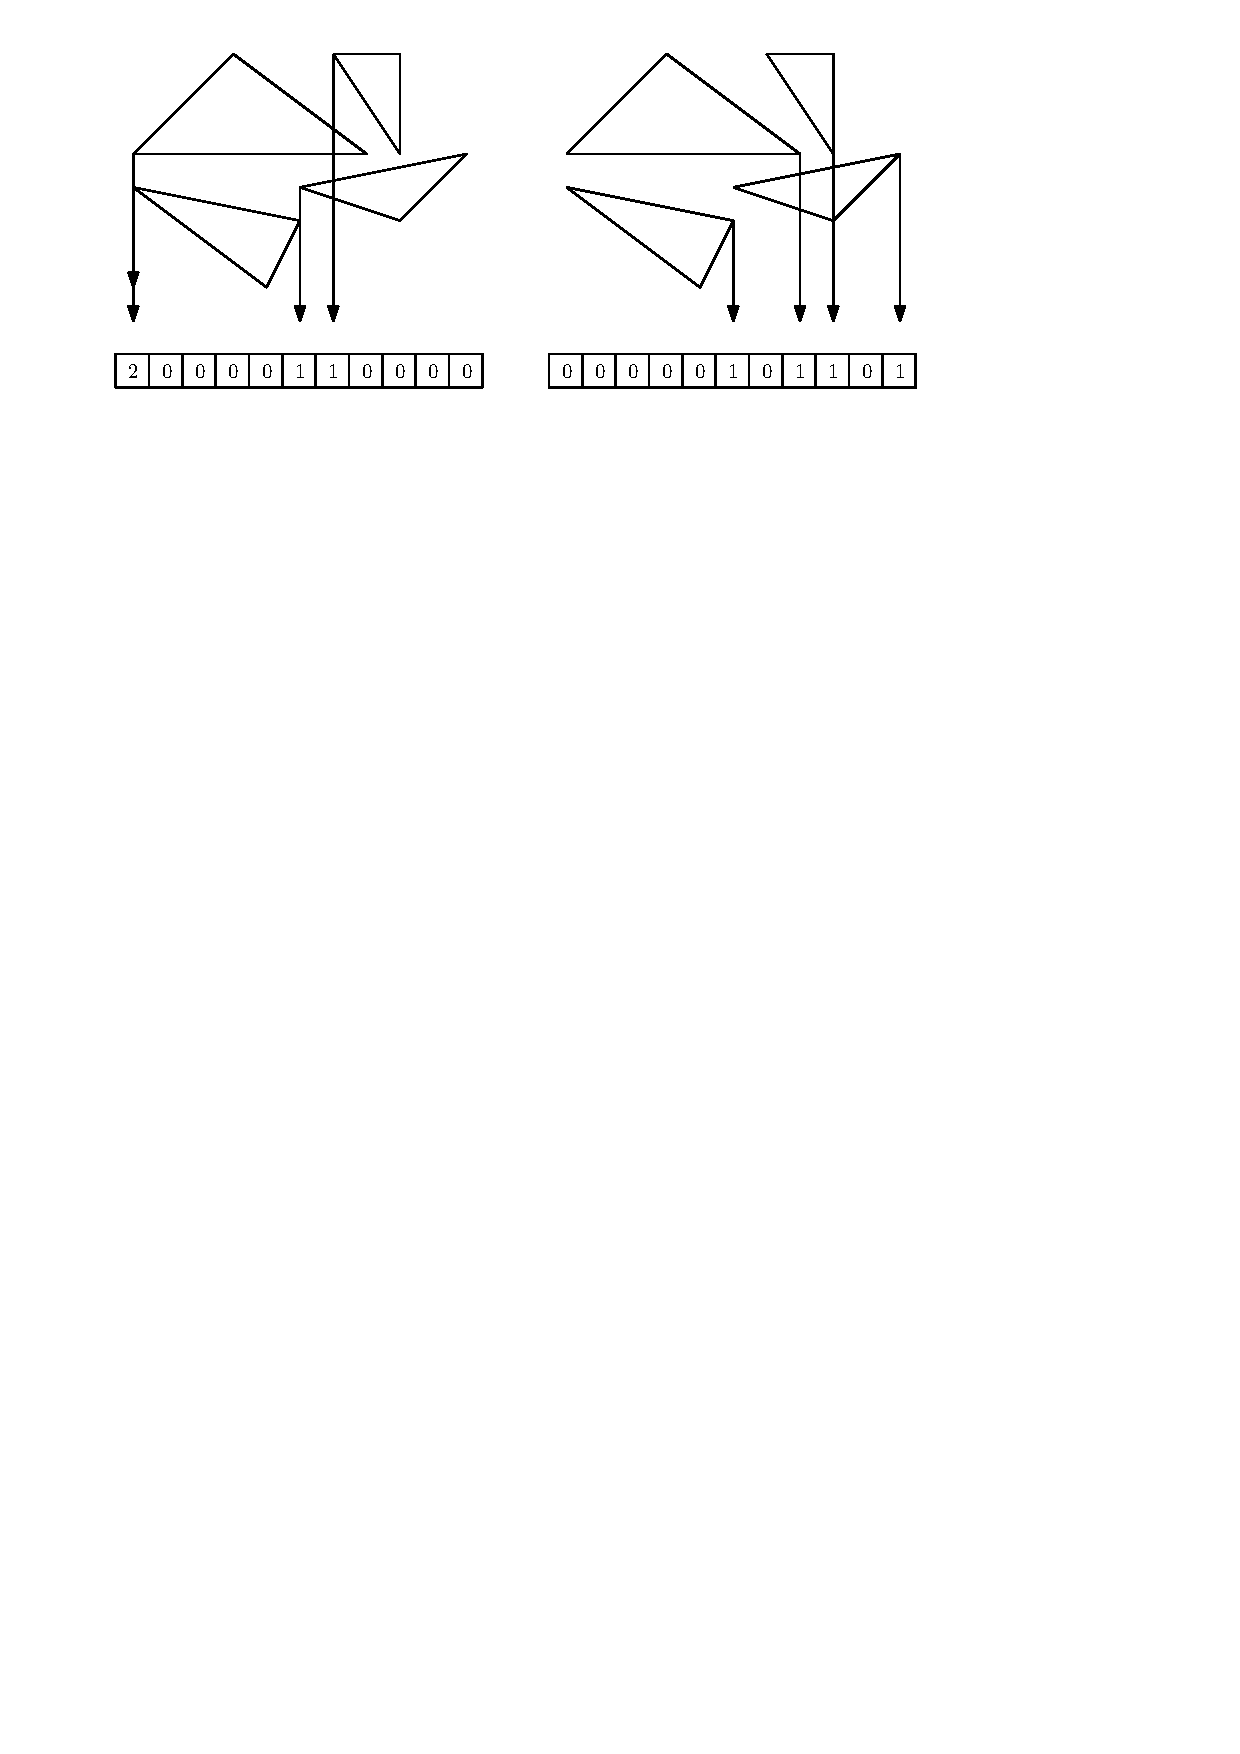
\includegraphics{figs/binning}
  \caption{\textit{Initializing the two bin sets for starts and ends of triangles. This will be done at the same time.}}
  \label{fig:binning}
\end{figure}
\begin{figure}
\centering
  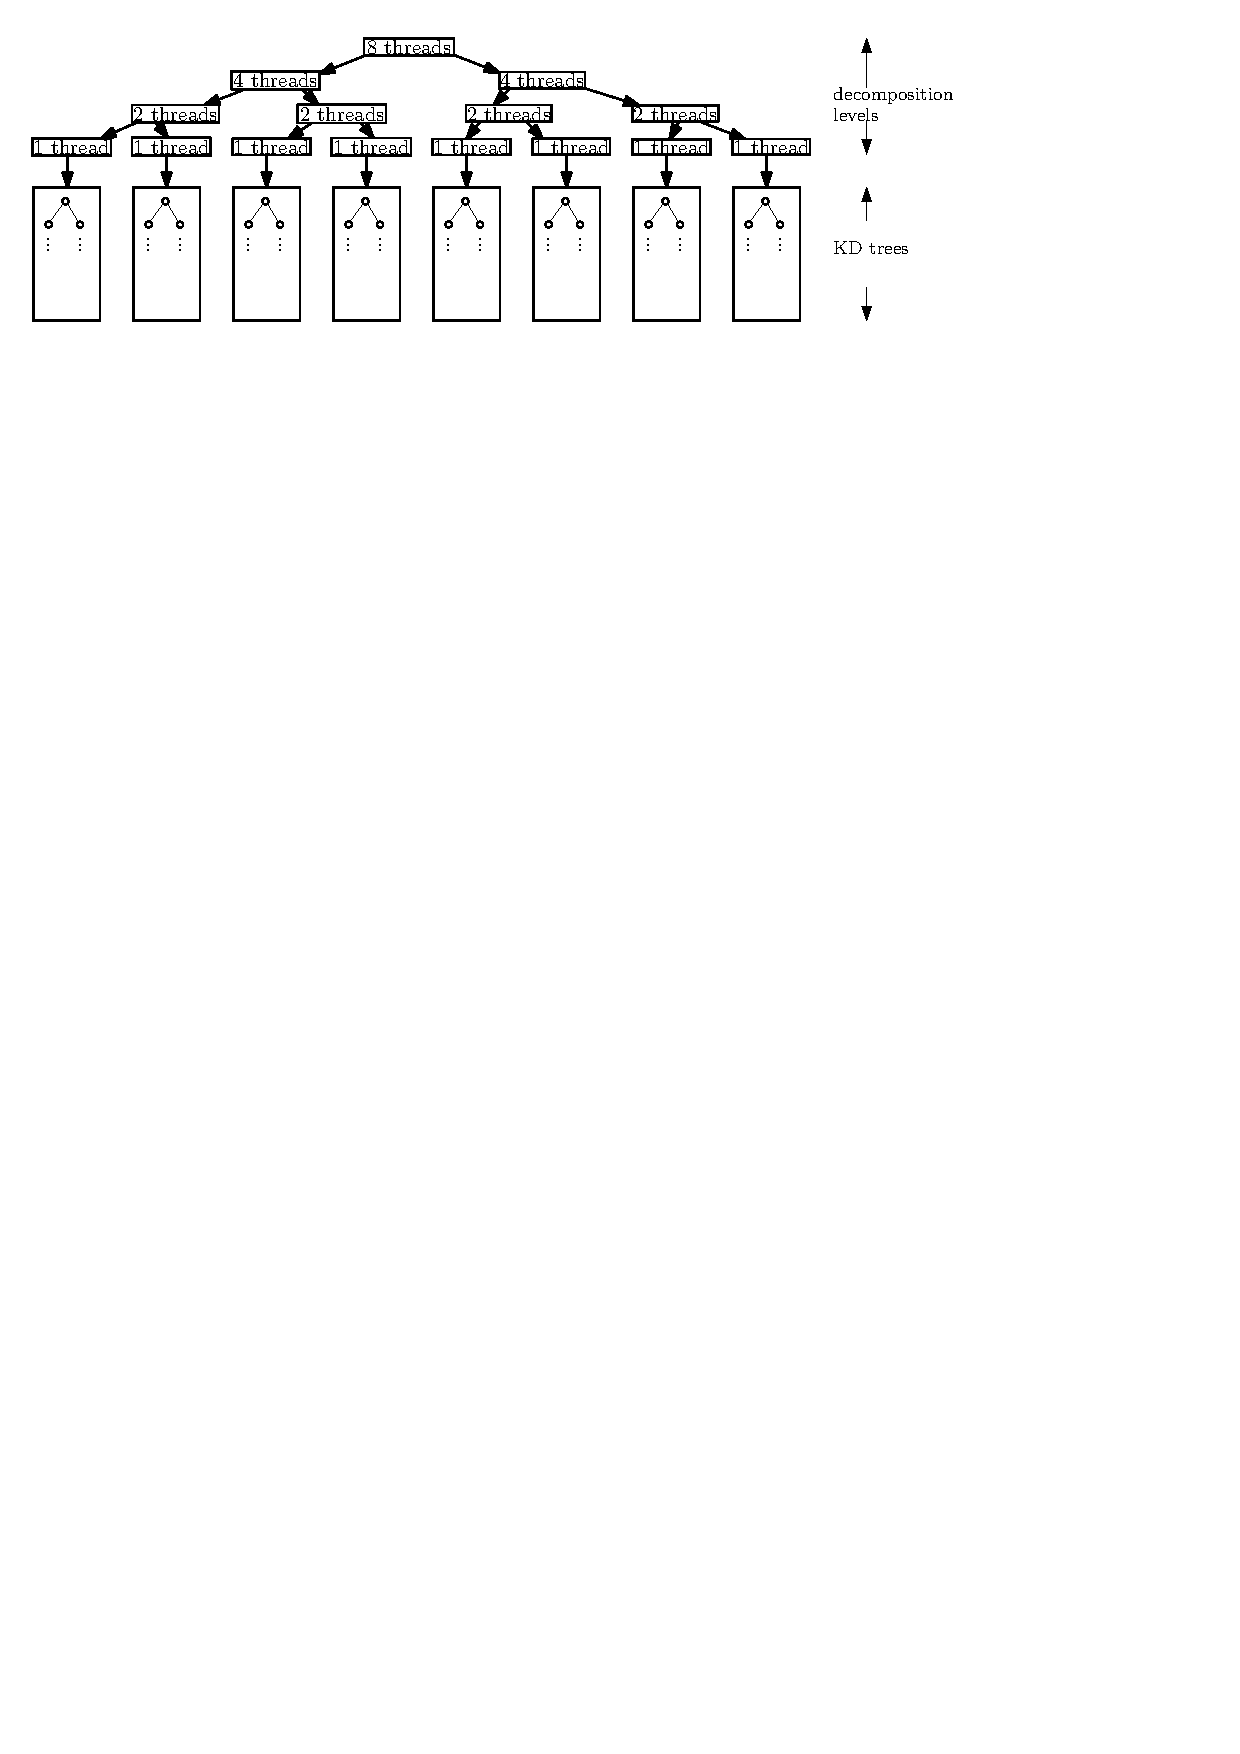
\includegraphics{figs/decomp}
  \caption{\textit{The space is decomposed until each thread gets its own tree.}}
  \label{fig:decomp}
\end{figure}
\begin{table}
\centering
\begin{tabular}{|l|l|l|}
\toprule
Scene & (Wald) & (Shevtsov) \\
\midrule
Buddha & 32.3 & 0.696\\
Bunny & 4.8 & 0.104\\
Dragon & 23.9 & 0.751\\
\bottomrule
\end{tabular}
\caption{\textit{Time to image in seconds. The algorithm by Shevtsov et al. \cite{hunt2006fast} and the $O(N\log N)$ algorithm by Wald and Havran \cite{wald2006building}, times taken from \cite{hunt2006fast}.}}
\label{table:13comp}
\end{table}

\section{Conclusion}
In this work we presented three algorithms for constructing KD trees for ray tracing. The first one by Wald and Havran \cite {wald2006building} is a beautiful theoretical algorithm that pushed the complexity for exact SAH KD trees to its lower bound. It is a famous algorithm, referenced and compared in many papers. It put a good foothold in the world of KD trees with its precise complexity analysis and performance. The second algorithm by Hunt et al. \cite{hunt2006fast} approached the problem from a different angle, opting to approximate the SAH in order to decrease the tree construction time. This is going to be what a lot of future algorithms focus on, to be able to more efficiently calculate dynamic scenes. The algorithm by Shevtsov et al. \cite{shevtsov2007highly} is no exception. It provides an aggresive SAH approximation to achieve low tree construction times, allowing for much easier generation of dynamic scenes. This is also made possible by its novel paralellization techniques which could be expanded to different algorithms as well. All of these algorithms could also be used in conjunction with other optimization techniques such as MLRTA \cite{reshetov2005multi} for even better ray tracing performance.\\
\indent The important thing to conclude, is that these algorithms are not just standalone black boxes, they contain novel ideas which can, and have been expanded into new algorithms and new approaches. The field of ray tracing is ever-growing, and many algorithms and techniques are invented every year and it is important to understand some of the techniques that helped get it to where it is today, so we can continue to advance it in the future.

\newpage
% \bibliographystyle{abbrv}
% \bibliographystyle{IEEEtran}
\bibliographystyle{unsrt}
\nocite{*}
\bibliography{references}
\end{document}